
\chapter{DriveSense: Practical Driving Analytics with Smartphone Sensors} 
\label{chapter_drivesense}

Sensing various driving behaviors, such as accelerations, brakes,
turns, and change lanes — is of great interest to many applications,
e.g., understanding drive quality, detecting road conditions, and
more. Many such applications rely on using smartphone placed in a
vehicle to collect such data for ease of deployment and use. However,
several driving analytics techniques in the recent past, including
our own, make simplifying assumptions that the smartphone is
stably fixed with certain orientation and the car is driving on flat
roads. Our deployment experience reveals that existing approaches
may cause orientation misalignment and acceleration over/under
estimation due to road slopes and human interactions, which lead
to significant sensing errors for driving analytics applications.
In this chapter, we present a smartphone app called DriveSense,
which addresses these challenges and conduct driving analytics
accurately by using various smartphone sensors.  


\section{The Problems}


Smartphone inertial sensors are used for driving analytics. 
The IMU accelerometer measures 3D acceleration 
\footnote{Depending on context, acceleration refers to either the 
rate of change of velocity per unit of time or the driving behavior
when the driver press the gas pedal.} 
changes and can be used to detect accelerations and brakes. 
The IMU gyroscope measures 3D angular change and can be used
to detect steering motions such as turns and lane changes.
Existing driving analytics approaches \cite{wang2013sensing,hansenspeed,chen2015invisible} 
assume ideal scenarios, i.e., 
the car is moving on flat road and  
the smartphone is stably mounted
with fixed relative orientation to the car. 


In trying to relax such assumptions, 
we found that the accuracy of inertial sensors, 
especially the accelerometer, are sensitive to road conditions, 
orientation changes and mounting stability (as a result of human interactions). 
We start with an example trip to illustrate the 
\emph{acceleration over/under estimation} problem
due to slopes and the effects of gravitation.  
We show that existing coordinate alignment
method may cause \emph{coordinate misalignment}. 
Such problems cannot be easily fixed due to 
the low accuracy of inertial sensors. 
We also discuss unmanaged smartphone usage
cases and the impacts on driving analytics, 
i.e., relative orientation changes and the 
smartphone is not stably mounted. 

\subsection{Sensitive to Road Conditions}

\subsubsection{Acceleration Over/Under Estimation}


\begin{figure}[!tbp] \centering
    \begin{subfigure}[b]{\linewidth}
         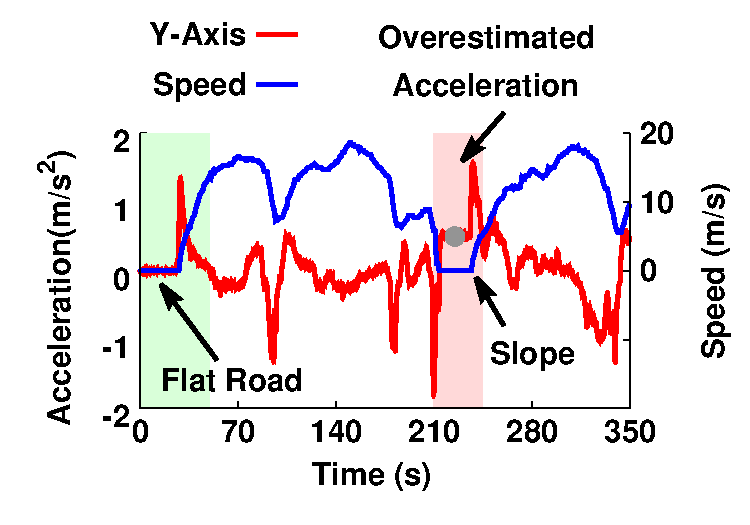
\includegraphics[width=3.3in,angle=0]{Figs/DriveSense/slopeaware/motivation.pdf}
         \vspace{-0.4cm}
         \caption{The accelerometer y-axis (along the car's heading direction) and OBD speed readings.}         
        \label{motivation:a}
    \end{subfigure} %

    \begin{subfigure}[b]{\linewidth}    
        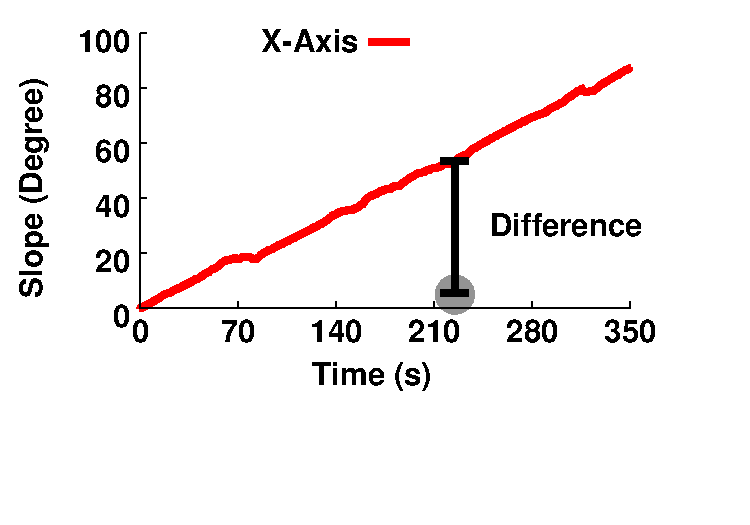
\includegraphics[width=3.3in,angle=0]{Figs/DriveSense/slopeaware/gyro_motivation.pdf}
        \vspace{-1.5cm}
        \caption{The accumulated gyroscope x-axis (tracking car's rotational speed when going upslope/downslope) readings.}
        \label{motivation:b}    
    \end{subfigure} 
\caption{Sensor and OBD data from the motivation example trip.}
\label{motivation}
\vspace{-0.2cm}
\end{figure}



We collect an example driving trip with various driving activities 
such as brakes and accelerations using a LG Nexus 5.
Before the trip, we park the car in a flat parking lot and fix
the smartphone with a frame mounted between the driver seat
and the passenger seat.
The coordinates of the phone are manually aligned (as precisely as we can) with the car. 
We use a customized Android application to record the sensor data and OBD speed data.
The sensor and OBD data traces of the trip are illustrated in Fig. \ref{motivation}.
As can be seen from the figure, the trip started on a flat road
and the speed was $0m/s$ with acceleration $0m/s^2$. 
At time $210s$, there is a stop as the OBD speed reading was $0m/s$ 
while the accelerometer reading is around $0.5m/s^2$ indicating
the car is accelerating. It is an overestimated acceleration
due to road slope.
This is because the y-axis of the accelerometer can sense the gravity. 
The gravitational force may have an incremental or decremental effect
on the estimation of vehicle motion parameters. 
For example, a misalignment of five degrees may cause $0.85m/s^2$ 
acceleration estimation error.
For reference, the \emph{Snapshot Program} \cite{snapshot} records a hard brake if the deceleration is around $3m/s^2$.
Therefore, we conclude that \emph{road slopes and associated gravitational effect
cause acceleration over/under estimation}. 


\subsubsection{Accumulated Gyroscope Errors}

The gyroscope can be used to track three-dimensional angular changes
and is an ideal input for slope estimation. 
However, it is known to suffer accumulated errors \cite{zhou2014use}. 
As illustrate in Fig. \ref{motivation}, 
we observe similar error accumulation in our motivation experiment. 
The dark dot is the slope gradient calculated by the accelerometer.
The curve of gyroscope measures the accumulated angular changes  
when the car was driving upslope/downslope.
Intuitively, the accumulated angular change of gyroscope can be used to 
estimate the slope gradients.
Clearly, the accumulated error is much higher than 
the actual accumulated slope gradients estimated by the accelerometer. 
We refer interested readers to \cite{chen2015invisible, zhou2014use},  
for detailed gyroscope three-dimensional readings 
and corresponding vehicle movement. 
Since we only focus on going upslope/downslope, we are interested in 
x-axis gyroscope readings of the car (or aligned smartphone) only.
There are several reasons why we see accumulated errors of gyroscope. 
The first one is the constant drifts, where the gyroscope reading is 
not zero in still due to limited hardware precision.
As the angular changes add up, the constant drifts accumulate correspondingly, 
which leads to a rough linear function between accumulated error and time.
The second one is the vibration of the vehicle, which accelerates
the drifts of the gyroscope readings.
Misalignment (caused by either manual alignment in our experiment 
or the coordinate alignment algorithm) between the car and the smartphone can also introduce accumulated errors. 
This is because the x-axis of the gyroscope can also sense car's steering angular change like turns and lane changes
when the smartphone is misaligned with the car.

\subsubsection{Coordinate Misalignment}

\begin{figure}[!htbp]
\begin{center}
  \vspace{-0.2cm}
  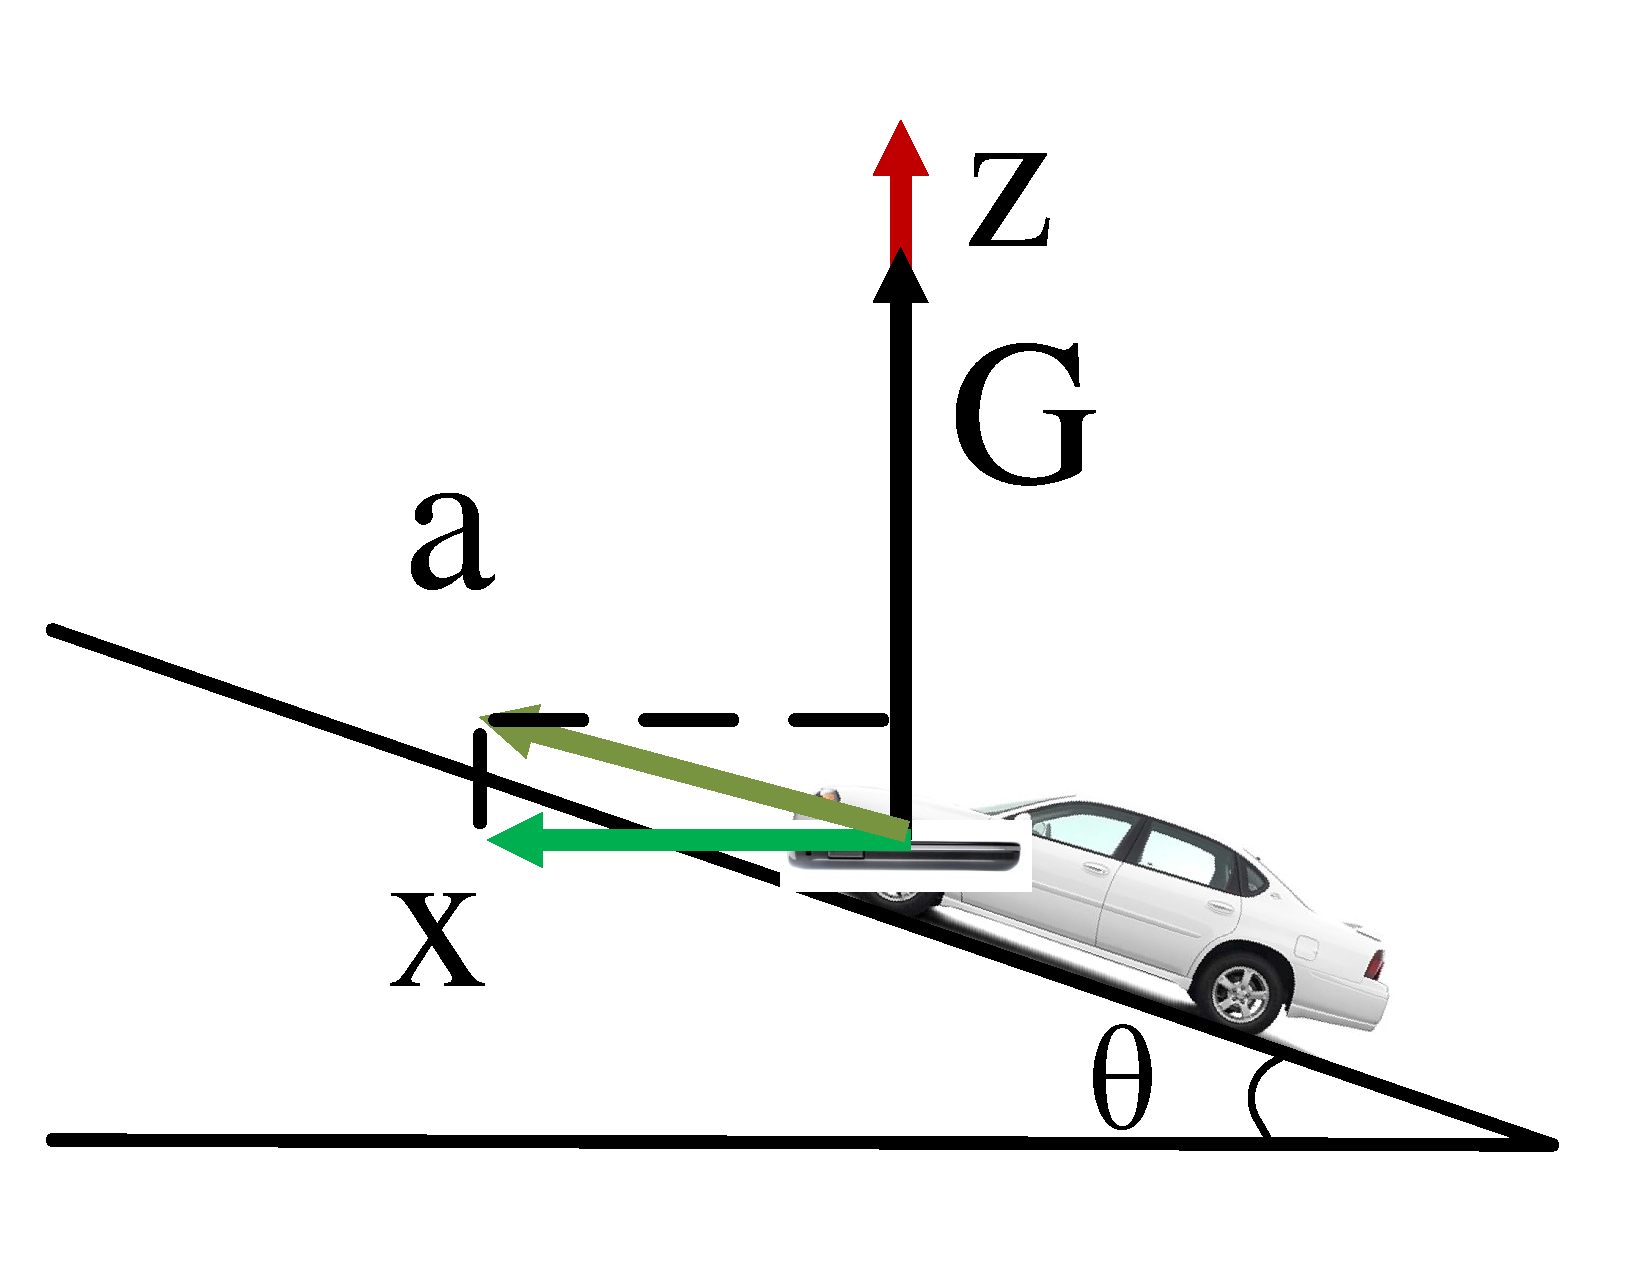
\includegraphics[width=2.6in, angle=0]{Figs/DriveSense/slopeaware/misalignment.pdf}
\vspace{-0.2cm}
\caption{Coordinate misalignment caused by road slopes.}
  \label{slopemisalignment}
\vspace{-0.4cm}
\end{center}
\end{figure}

Coordinate alignment is the process to align the
coordinates of the smartphone to those of the car 
\cite{hansenspeed, wang2013sensing, chen2015invisible}. 
We find that slopes cause misalignment
if the coordinate alignment is conducted on slope. 
Coordinate misalignment refers to the case when the aligned coordinates of 
the smartphone is not perfectly aligned with the coordinates of the car. 
Since the accelerometer can sense gravity, a misalignment
may also cause acceleration over/under estimation problem. 
As illustrated in Fig. \ref{slopemisalignment}, 
the car is moving upslope while the coordinate alignment algorithm
assumes the car is moving on flat road, 
which leads to the intersection angle $\theta$ between
aligned coordinates of the smartphone and the coordinates
of the car. 
Such misalignment may cause acceleration over/under estimation
when the driver is driving on flat road. 


\subsection{Sensitive to Human Interactions}


Human interactions may change the 
relative orientation and mounting stability of the smartphone, 
which degrade the usability and accuracy
of inertial sensors. 
Relative orientation change refers to the
orientation change of the smartphone independent of
the movement of the car. 
Imaging a passenger pick up the phone from pocket
and answer a phone call, 
the movement of the smartphone is the addition of 
the movement caused by human interactions and vehicle movements. 
Mounting stability refers to the degree of fixation of the smartphone, 
i.e., the mounting stability when the smartphone is fixed in car mount
it higher than the case when the smartphone is put in the pocket. 


The relative orientation change causes the sensor
readings are too noisy to be used.
Suppose the smartphone is rotated horizontally 
180 degree, then the output of accleleromter 
is completely reversed, i.e., the smartphone
detects brake when the car is accelerating. 
To eliminate such errors, 
the rotation matrix should be
re-estimated for accurate output. 
Coordinate alignment is an expensive process, 
which we will discuss in details in later sections, 
and frequent coordinate alignment may lead to 
gray period where the inertial sensors
cannot used for driving analytics. 



Mounting stability is also an important factor when 
conducting driving analytics by using inertial sensors. 
When the user puts
the smartphone in the pocket,
the vibration of smartphone may add extra noises.
We advocate the use of a metric to quantify mounting stability
and understand the sensor accuracy under
various stability levels. 




\section{Sensing with Inertial Sensors}
\label{imusensors}


IMU sensors are used in many driving analytics 
applications \cite{hansenspeed, wang2013sensing, chen2015invisible}. 
However, existing work assume the car is moving on flat 
roads and the smartphone is stably mounted in the vehicle. 
Different from these work, we propose several novel
techniques to improve the accuracy and usability of inertial sensors
by detecting orientation change, modeling stability,  
conducting slope-aware coordinate alignment and linear
acceleration estimation in a more practical manner. 
We design a slope-aware solutions to conduct 
coordinate alignment and track linear acceleration
by removing the gravity component dynamically from the aligned accelerometer readings. 
Second, we use clustering techniques to detect 
relative orientation changes. 
Third, we use moving variance to model the mounting
stability of the smartphone and evaluate sensing accruacy
based on mounting statiblity. 

\subsection{Slope-Aware Alignment}
\label{slopeaware}


\begin{figure}[!tbph]
\vspace{0.0cm}
\hspace{-0.5cm}
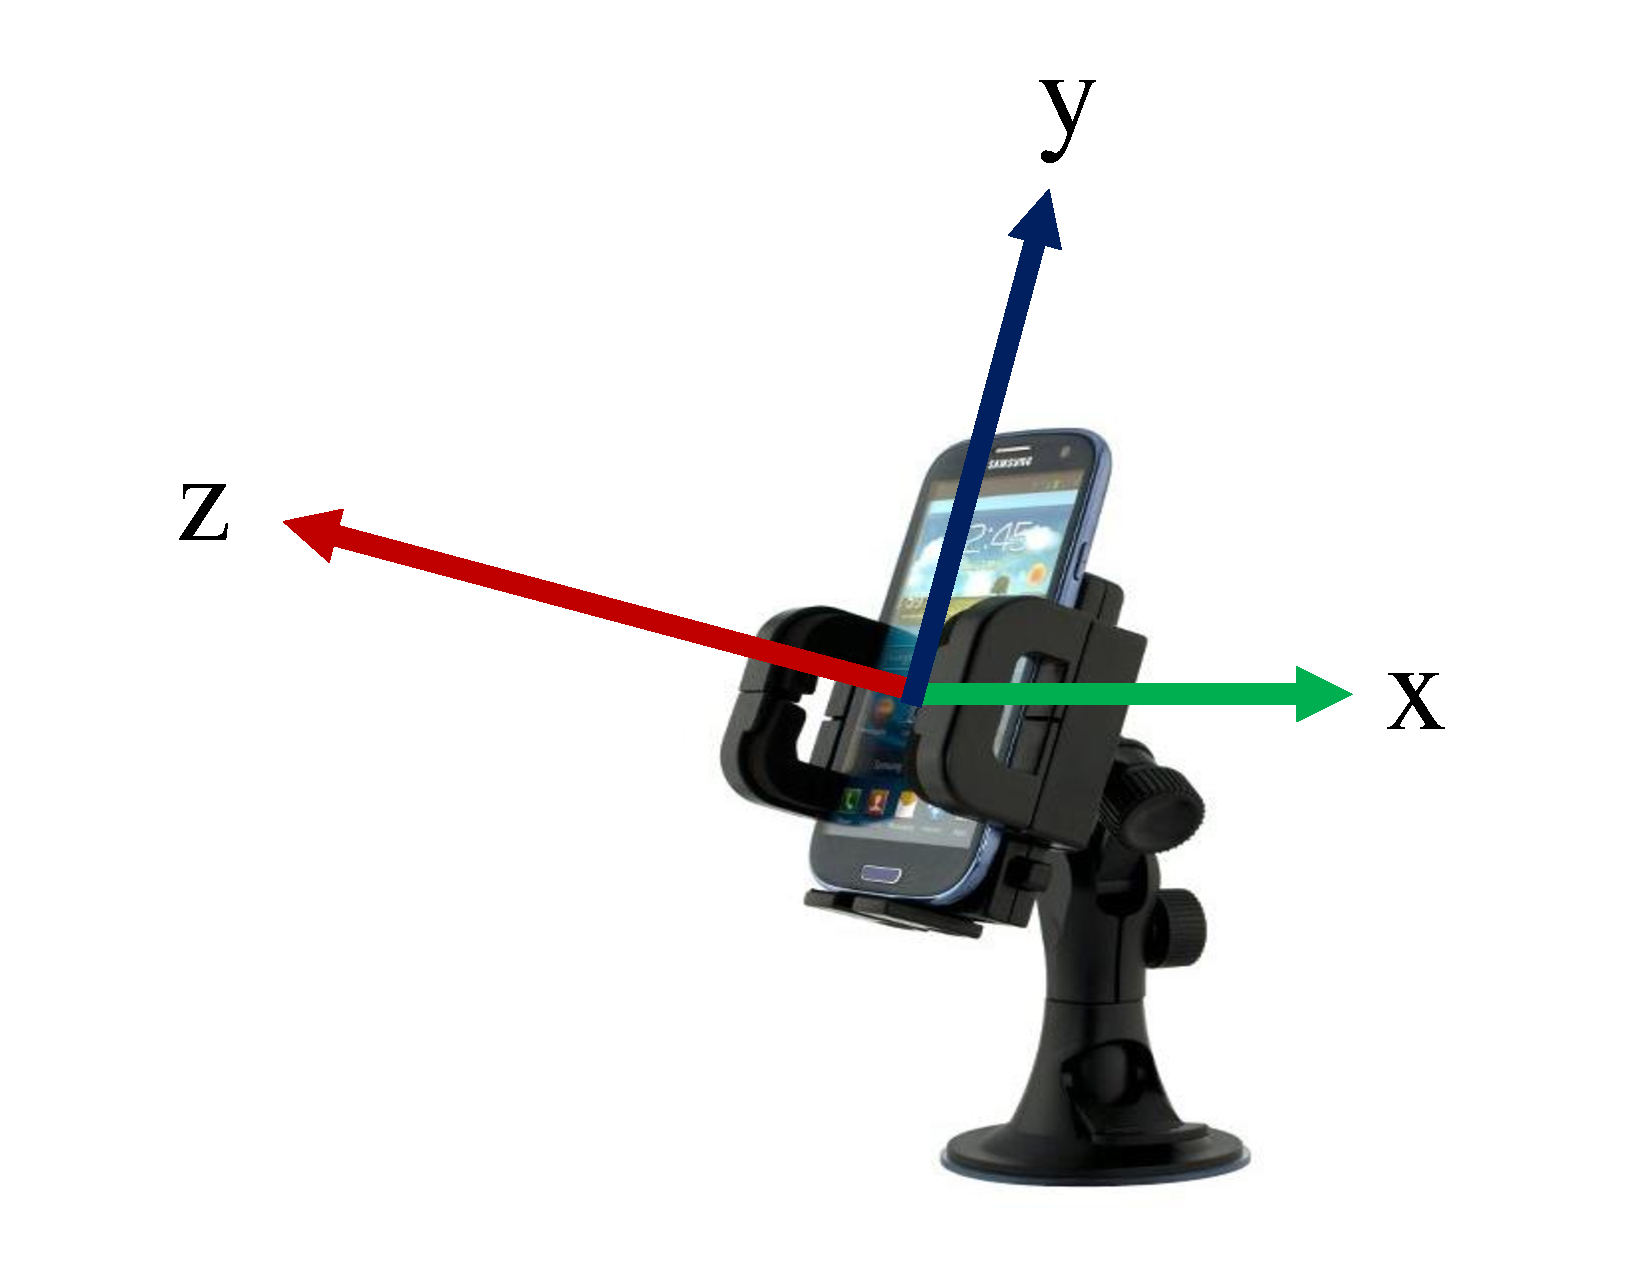
\includegraphics[width=1.8in,angle=0]{Figs/DriveSense/phone3d.pdf}
\vspace{0.0cm}
\hspace{-1.0cm}
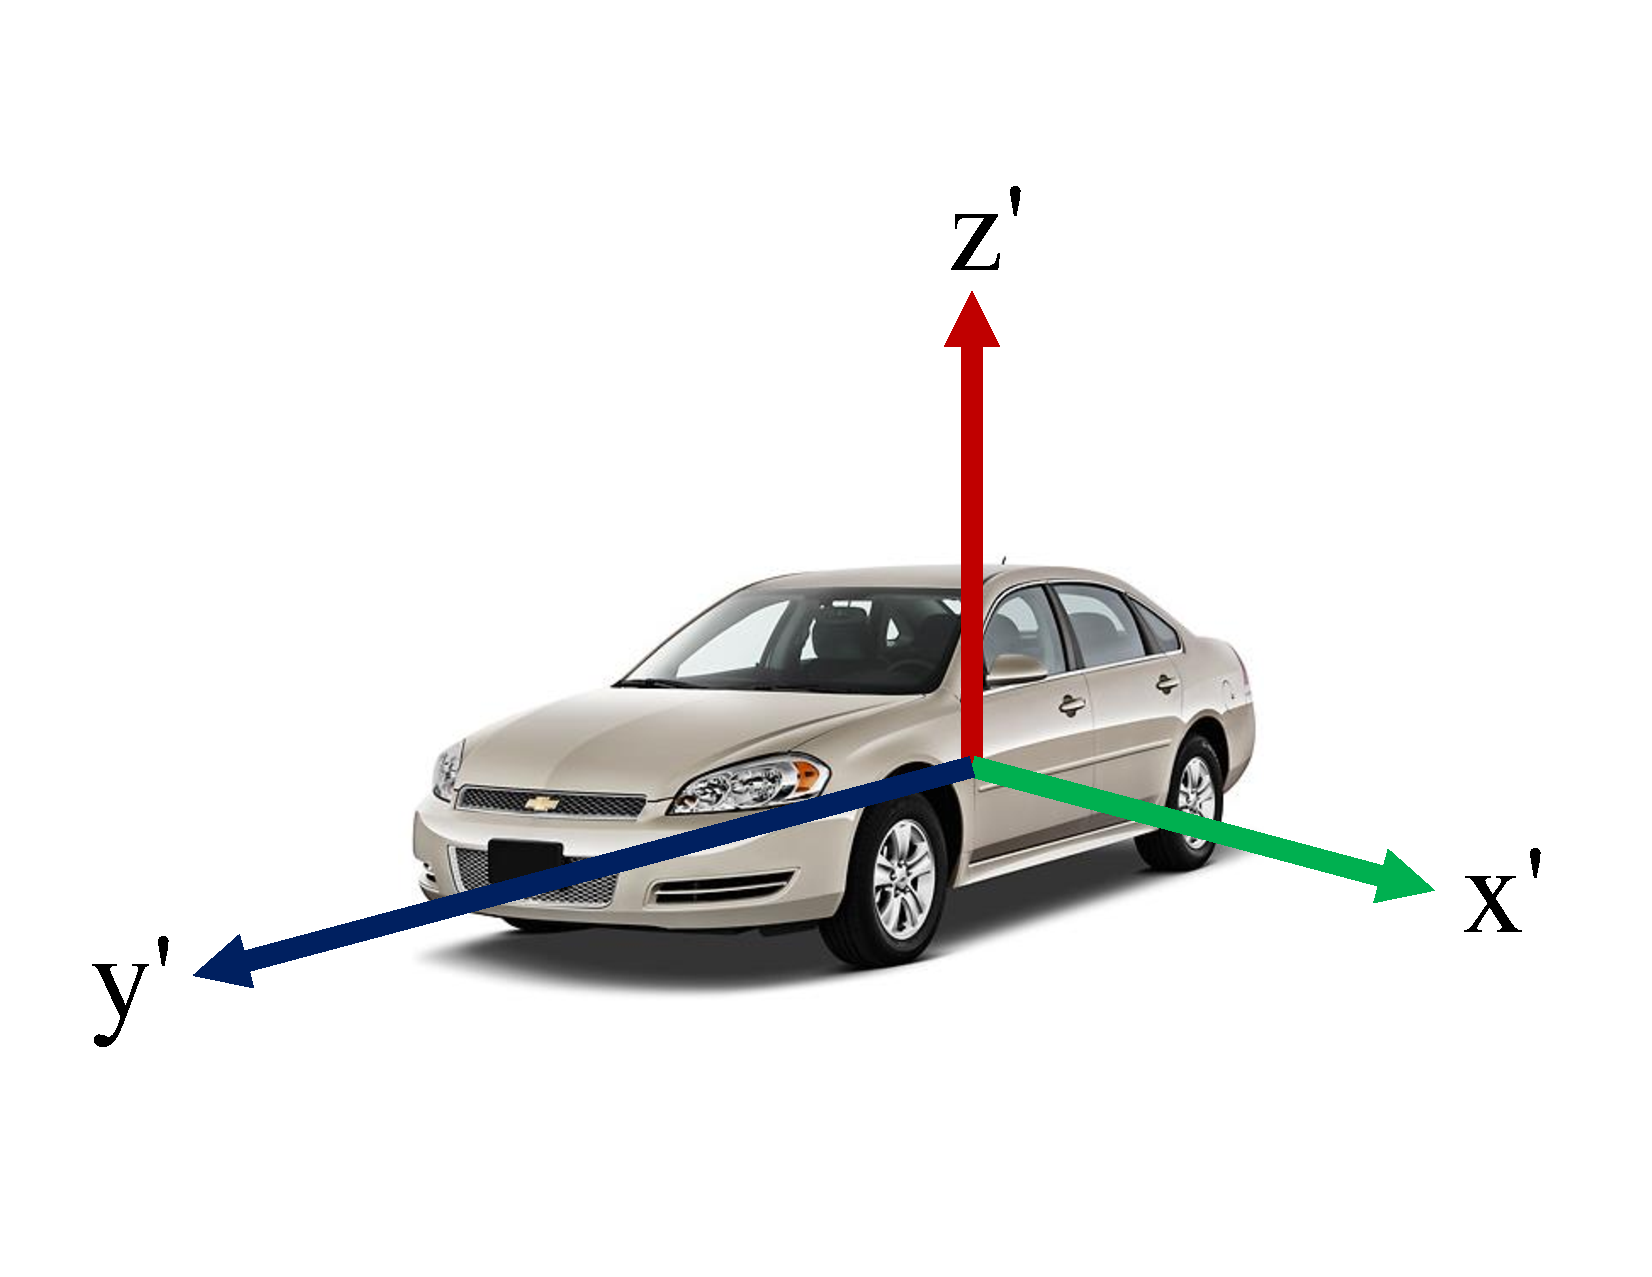
\includegraphics[width=1.8in,angle=0]{Figs/DriveSense/car3d.pdf}
\vspace{-0.2cm}
\caption{Coordinate system difference between a smartphone $[x, y, z]$ and a car $[x', y', z']$.}
\vspace{0.2cm}
\label{coordinates}
\end{figure}


\subsubsection{Slope-Aware Alignment and Linear Acceleration Estimation}


As illustrated in Fig. \ref{coordinates}, we use 
$[x, y, z]$ to represent the three dimensions of a smartphone
and use $[x', y', z']$ to represent the three dimensions
of a car. 
Coordinate alignment is the process that trains the rotation
matrix $R = [\hat{i}, \hat{j}, \hat{k}]$, 
where $\hat{i}$, $\hat{j}$ and $\hat{k}$ are three unit coordinate vectors,
so that $[x', y', z'] = [x, y, z] \times [\hat{i}, \hat{j}, \hat{k}]$.




\textbf{Step 1: Stop Points Extraction}. 

Identifying stop points are useful to conduct an initial alignment. 
We use a sliding window to track the deviation of the
accelerometer readings for this purpose.
The deviation is expected to be small when the car is stopped, 
i.e., in front of stop sign of red traffic light. 
But different cars have different vibrations, 
which affect the readings of the accelerometer. 
To identify a threshold for the deviation, 
we extract the stop points according to the speed information
collected from the OBD port.
We record the start time $s_t$ and end time $e_t$ that 
any speed reading in between is zero. 
To eliminate possible asynchronization and drifted value
after passing low-pass filter, 
we remove the points of the first 500ms and the last 500ms,
i.e., the data points within $[s_t + 500, e_t - 500]$. 
This process helps us to set the threshold to detect
stops. 
We only use OBD as a training input, 
our method can be used on any smartphone and vehicle settings
without OBD inputs. 
 

\textbf{Step 2: Horizontal Alignment}. 


Road slope affects the accuracy of coordinate alignment
in each step. 
During horizontal alignment, a slope-aware alignment method can
be much more effective than a slope-unaware approach. 
As illustrated in Fig. \ref{direction}, 
slope-unaware solutions assume all the data points 
pass the origin point and try to fit all the data
points for a single fit curve, 
while slope-aware solution treats each road segment
as different inputs (deviating from the origin point
due to slopes) and combine to improve the accuracy. 

To train the rotation matrix, we need to select the segments that the car is moving 
straight, and estimate the angle between the 
heading direction and the smartphone's horizontal coordinates \cite{wang2013sensing}.
To derive the rotation matrix from discrete sensor data points, 
we need to fit the curve and find the direction unit vector. 
We propose to train the horizontal
unit vector for each segment and combine each training results gradually with different weights.
There are lots of straight driving segments as illustrated in Fig. \ref{direction}, 
but not all of the segments are good for the training purpose. 
Each segment is selected based on the number of data points that
indicate the car is moving.
The intuition is that more data points could be more statistical significant. 
In Fig. \ref{direction}, we separate four segments and train the 
horizontal unit vector separately.
Clearly, this approach gives better view results that the four slopes of the 
fitting curves are $-0.98$, $-0.87$, $-0.93$ and $-0.95$, respectively. 
The weighted average is $-0.94$. 
After obtain the angle $a$, the horizontal 
rotation matrix can be calculated as follows. 

\[
R_h
	=
\begin{bmatrix}
   cos(\alpha) & -sin(\alpha) & 0 \\
   sin(\alpha) & cos(\alpha) & 0 \\
   0 & 0 & 1
\end{bmatrix}
\]



\begin{figure}[!tbph] 
\hspace{-0.4cm}
  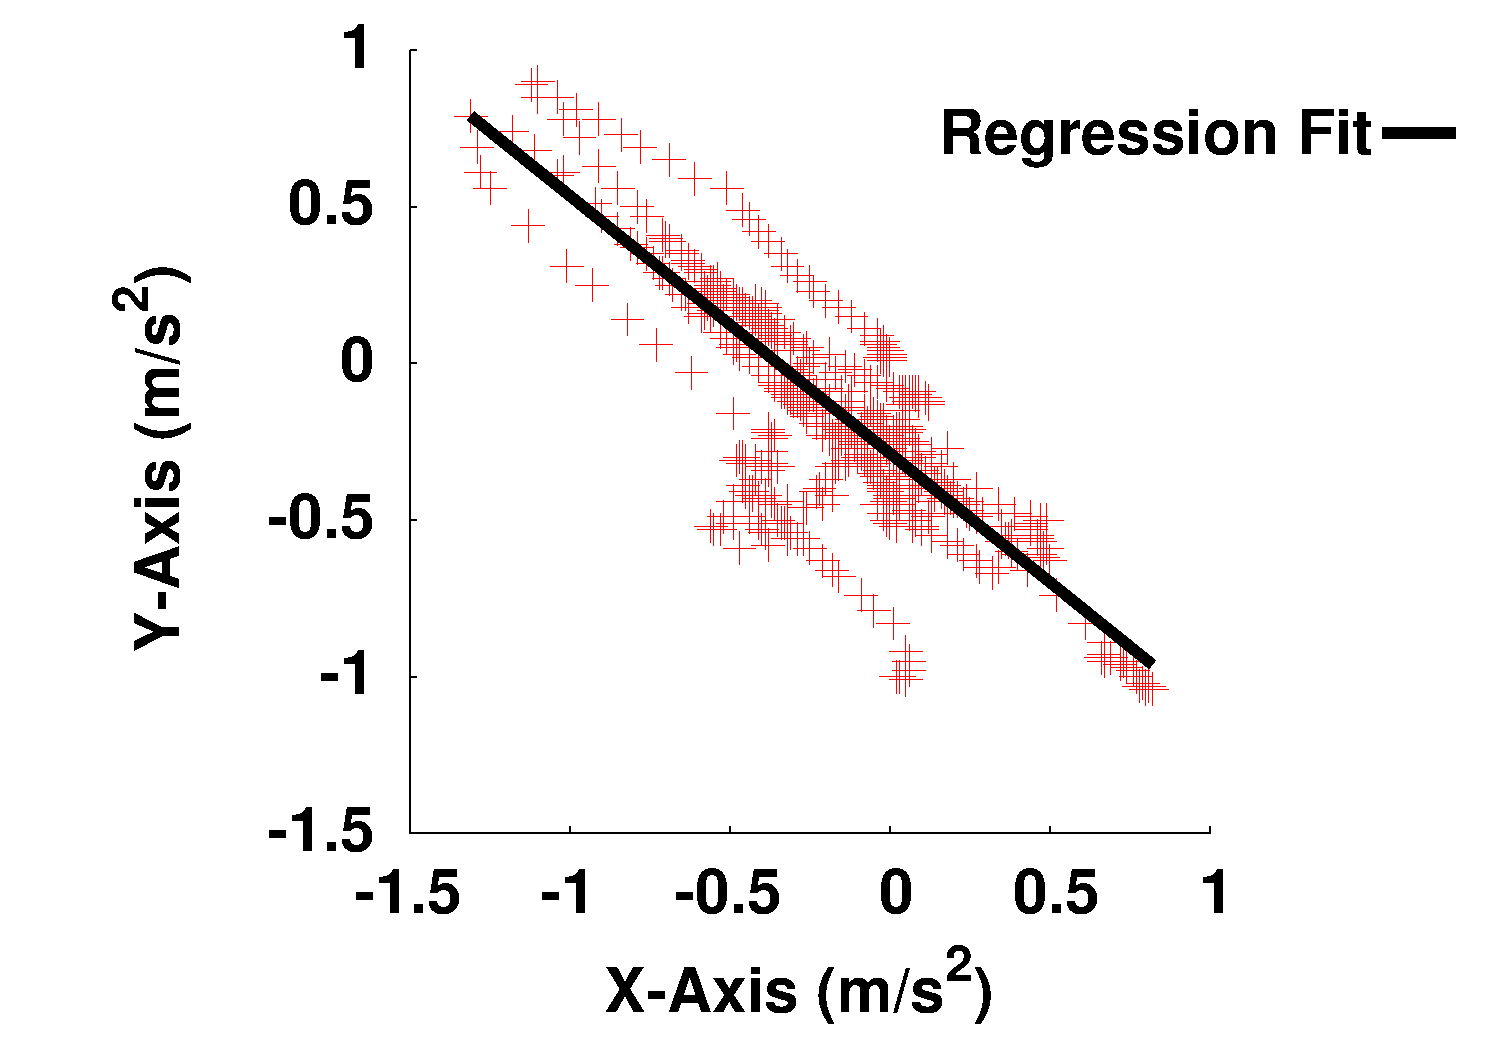
\includegraphics[width=2.6in,angle=0]{Figs/DriveSense/slopeaware/stateoftheart.pdf}
\hspace{-0.0cm}
  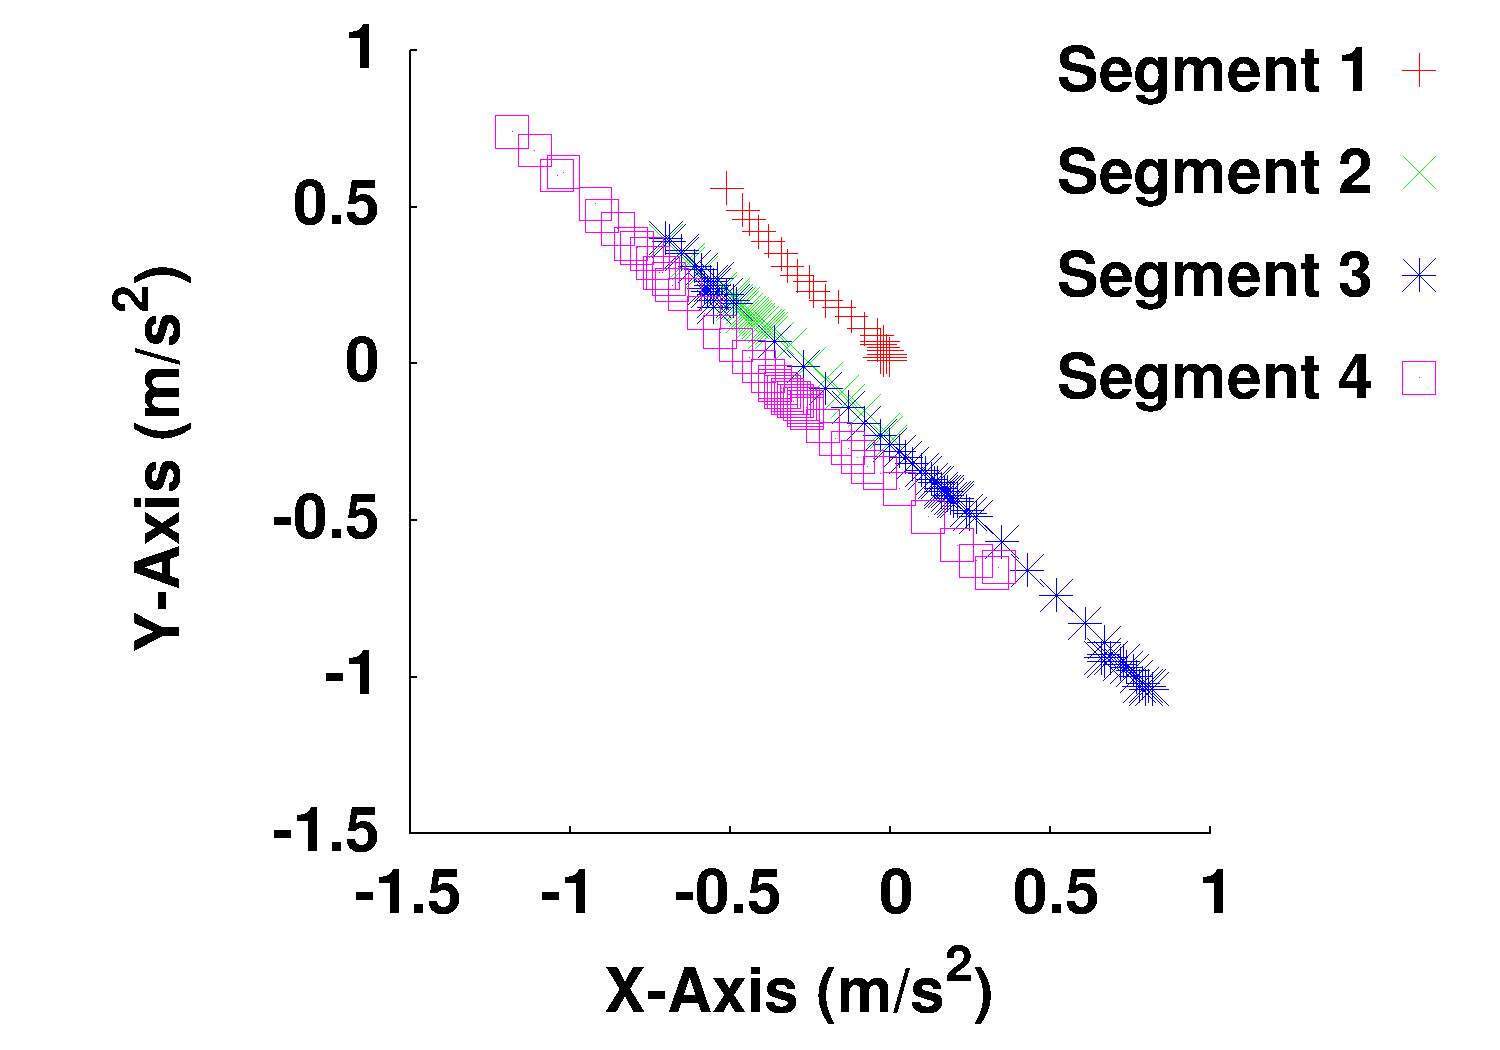
\includegraphics[width=2.6in,angle=0]{Figs/DriveSense/slopeaware/direction.pdf}
\hspace{-0.0cm}
   \caption{Training horizontal rotation matrix by using traditional
approach (above) and slope-aware multi-segment method (below).}
\label{direction}
\vspace{0.4cm}
\end{figure}





\begin{figure}[!htbp]
\begin{center}
%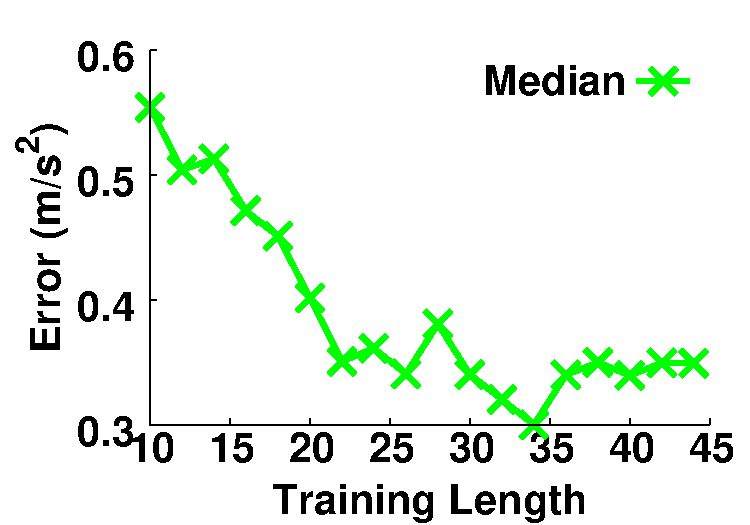
\includegraphics[width=1.7in,angle=0]{Figs/DriveSense/trainlengthanderror.pdf}
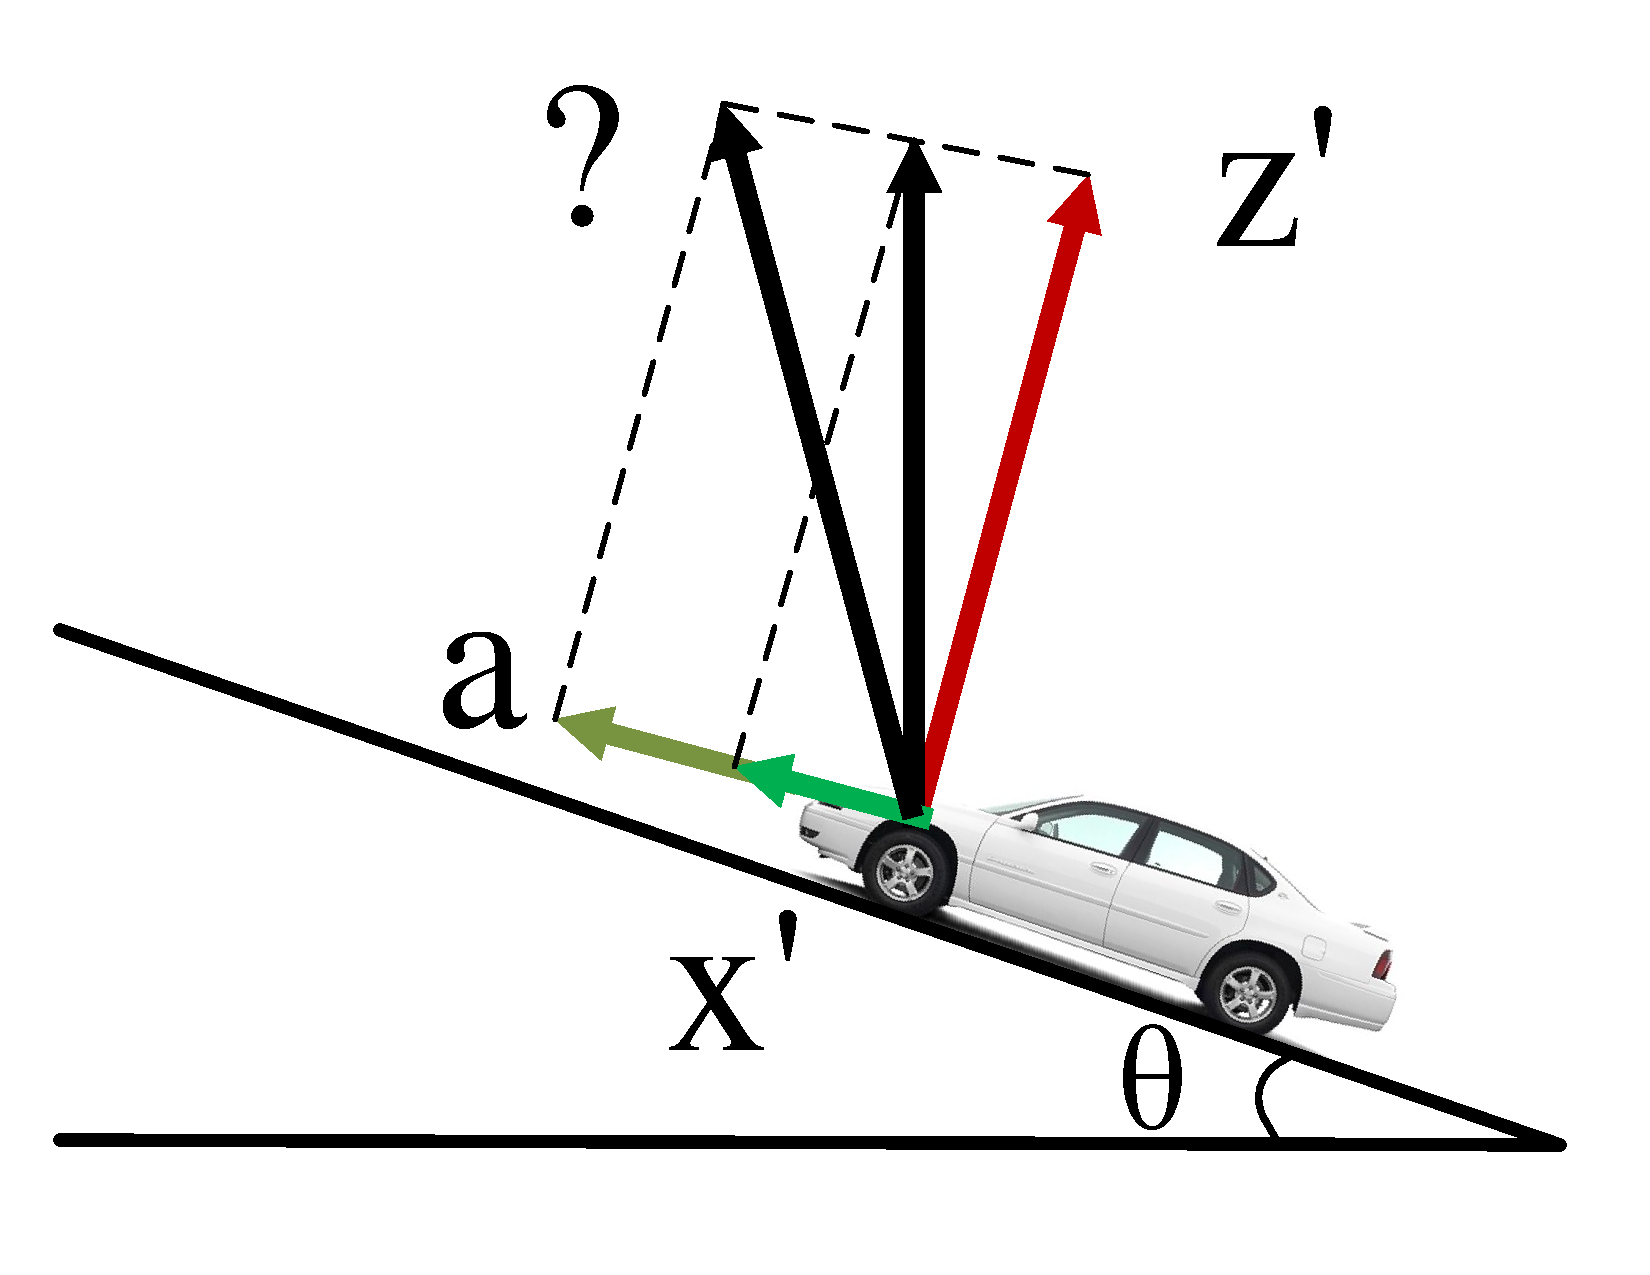
\includegraphics[width=2.0in, angle=0]{Figs/DriveSense/uncertain_vertical.pdf}
\vspace{0.0cm}
	\caption{
Since the actual acceleration of the car 
and the component of gravitational force (along the slope) are unknown, 
the direction of force is uncertain when conducting vertical alignment.
}
\label{training}
\vspace{0.4cm}
\end{center}
\end{figure}



\begin{algorithm}
\caption{Angle Search Algorithm}
\label{search}
\begin{algorithmic}[1]
\Input{$D_a$: The 2D accelerometer data after horizontal alignment}
\Output{$\theta_{o}$: The best fit angle}
\Procedure{AngleSearch}{}
\State $dev_{min} \gets MAX$;
\State $D_{t} \gets []$;
\For{$\theta$ \texttt{in} (-$\alpha$, $\alpha$)}
\For{$[y_i, z_i]$ \texttt{in} $D_a$}
\State $M_\nu$ $\gets$ $\begin{bmatrix}\cos\theta & -\sin\theta\ \\ \sin\theta & \cos\theta \end{bmatrix}$;
\State $[y'_i,z'_i]$ $\gets$ $[y_i,z_i]* M_\nu$;
\State $D_t.push(z'_i)$;
\EndFor
\State $dev_x \gets deviation(D_t)$;
\If {$dev_x < dev_{min}$}
\State {$dev_{min}$ $\gets$ $dev_x$};
\State {$\theta_{o}$ $\gets$ $\theta$};
\EndIf
\EndFor
\Return $\theta_{o}$;
\EndProcedure
\end{algorithmic}
\end{algorithm}
\vspace{-0.6cm}


\textbf{Step 3: Slope-Aware Alignment}. 

Estimating road slope at alignment time is challenging. 
In horizontal alignment, we can fit a curve as the moving
direction of the car (or the direction of force) is fixed and not much interfered 
by gravity. 
In vertical alignment, however, the direction of force is changing. 
As illustrated in Fig. \ref{training}, the direction of force changes
as the change of the acceleration of the car. 
There are two parameters are unknown, the slope gradient 
and the vehicle acceleration. 
The vehicle acceleration varies at each data point, 
which varies the direction of force and makes it is very
challenging to estimate the parameters.
We use one heuristic searching algorithm to search for best alignment angle. 
The algorithm relies on the property that the $z'-axis$ of 
the car should be constant over the same slope. 
Firstly, we assume the horizontal alignment is complete and
we convert a 3D alignment problem into a 2D alignment problem. 
The two dimensions are $y-axis$ and $z-axis$, 
as illustrated in Fig. \ref{training}.
By iterating over all the possible angles, 
we calculate deviation of the $z'-axis$ and locate the one with the least deviation. 
The pseudo code of the search algorithm is illustrated in 
Form \ref{search}.




\textbf{Step 4: Linear Acceleration Estimation}.



\begin{figure*}[t]
\begin{center}
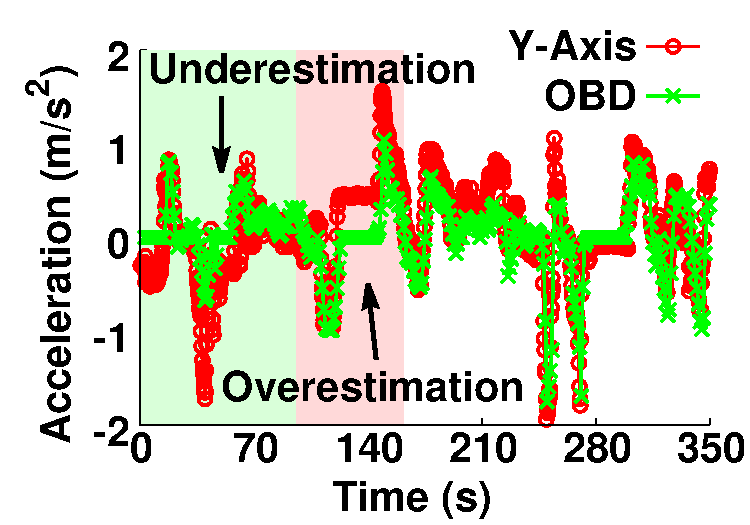
\includegraphics[width=2.2in,angle=0]{Figs/DriveSense/slopeaware/accspeed.pdf}
\hspace{-0.0cm}
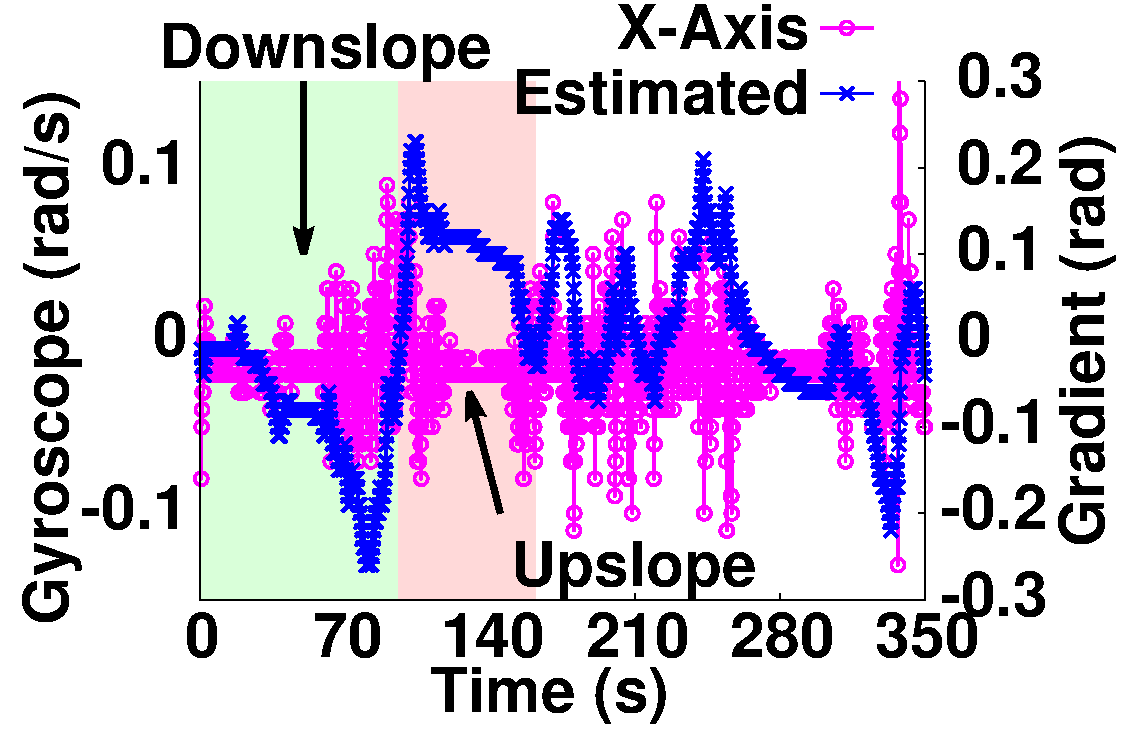
\includegraphics[width=2.2in,angle=0]{Figs/DriveSense/slopeaware/gyrocompare.pdf}
\hspace{-0.0cm}
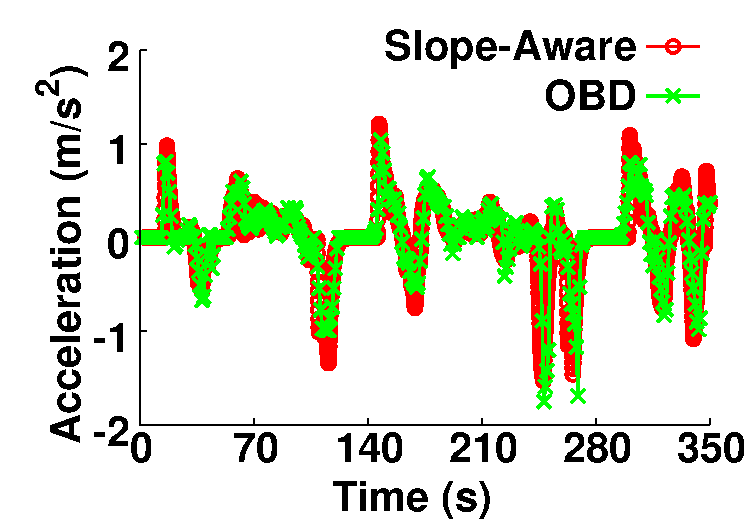
\includegraphics[width=2.2in,angle=0]{Figs/DriveSense/slopeaware/acccompare.pdf}
\hspace{-0.0cm}
\vspace{-0.2cm}
\caption{Slope-Aware coordinate alignment and linear acceleration estimation. 
The Figs/DriveSense are about acceleration over/under estimation caused by slopes (left), 
using gyroscope to estimate road slopes (middle), 
comparing estimated linear acceleration with groundtruth acceleration (right).}
\vspace{-0.2cm}
\label{linear_acceleration}
\end{center}
\end{figure*}


After coordinate alignment is complete, 
we can track the acceleration of a car by using the accelerometer's y-axis. 
We illustrate the acceleration values from aligned accelerometer 
in an example trip illustrated in Fig. \ref{linear_acceleration}. 
As the figure shows, comparing with the accelerations by OBD,   
the accelerations by the accelerometer of the first $90s$ 
are underestimated and the following $60s$ are overestimated.
This is because the car is moving mainly downslope and then mainly upslope. 
The deviated estimations may cause false positives/negatives on 
capturing driving behaviors such as brakes and accelerations.

We apply the same rotation matrix to the gyroscope data and 
illustrate the gyroscope x-axis data in Fig. \ref{linear_acceleration}.
After removing the constant drifts, 
it shows clear trends that the car is moving downslope and then
upslope.
Given the similar trends illustrated in two plots, 
we can estimate the slope gradient and deduct the gravitational force
components. 
We use similar calibration techniques proposed in \cite{zhou2014use}. 
We identify the road segments and stop points where accelerometer
can provide more accurate slope gradients to calibrate gyroscope.  



 

\subsection{Detecting Relative Orientation Change}


\begin{figure}[!htbp]
\begin{center}
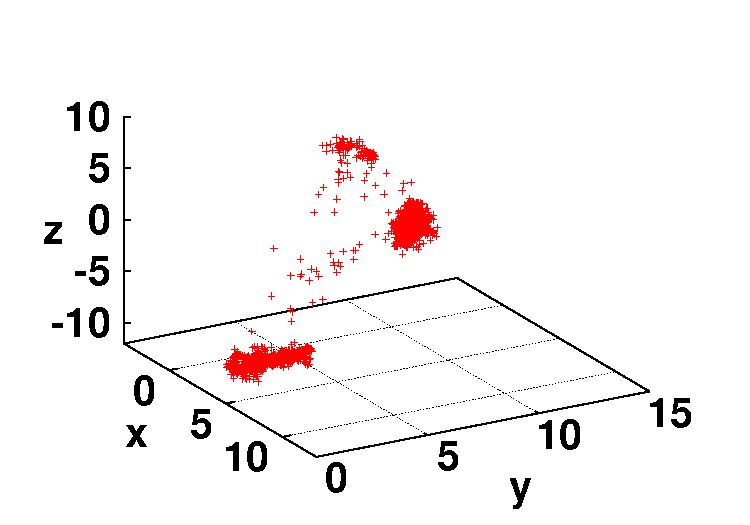
\includegraphics[width=1.7in,angle=0]{Figs/DriveSense/example_cluster.pdf}
\hspace{-0.8cm}
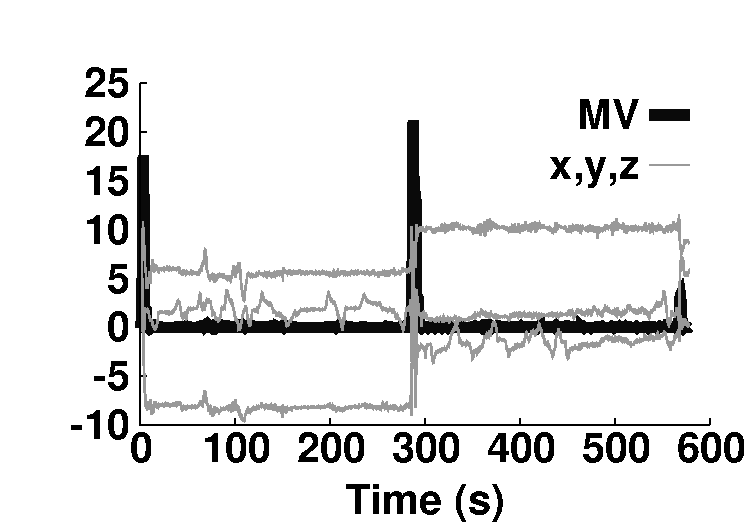
\includegraphics[width=1.7in,angle=0]{Figs/DriveSense/example_change.pdf}
\vspace{0.0cm}
\caption{The accelerometer data in one trip where the smartphone is picked up
from a pocket and put on the car mount holder. 
The upper cluster is formed when the user start the app at the beginning
and put the phone into the pocket, which is also detected by MV method. }
\vspace{-0.2cm}
\label{example_change}
\end{center}
\end{figure}


Using inertial sensors to estimate vehicle motions
is also vulnerable to smartphone relative orientation changes. 
Relative orientation refers to the relative orientation 
between the smartphone and the car.  
When the smartphone is fixed in the car and 
the car is moving upslope or making turns, the
relative orientation of the smartphone does not change 
as there is no relative movement between the smartphone
and the car.  
The relative orientation is usually changed by the smartphone
user, e.g., moving the smartphone from pocket to the car mount
for navigation.



The gyroscope is able to track absolute orientation changes
of the smartphone \cite{zhou2014use}. 
Tracking relative orientation change is a different. 
Since the smartphone is moving at the same pace 
with the car (suppose the smartphone is mounted), 
the gyroscope will sense the steering motions of the 
car, i.e., making turns, driving upslopes etc. 
It is challenging to separate the movement of the car
and the movement of the smartphone itself. 


We find accelerometer can be used to reliably detect orientation changes. 
While the movement of the car will introduce noises accelerometer
readings, but the noises are relatively small ($1-2m/s^2$ in most of the cases) 
in comparison to the gravitational force sensed by accelerometer. 
Once there is an orientation change, the gravity components
sensed by accelerometer are changed dramatically.
During one test trip, we move the smartphone
from pocket to car mount holder. 
The accelerometer sensor readings are illustrated in Fig. \ref{example_change}. 
All the accelerometer sensor readings can be naturally
classified into three clusters. 
The upper small one is formed when the user hold
the smartphone and manually start the app. 
The rest two are formed when the smartphone is in 
the pocket and on the car mount holder, respectively. 
Intuitively, incremental clustering methods are reasonable 
choices to identify orientation change, 
i.e., there is new cluster formed. 


\textbf{Incremental Clustering}. Traditional incremental clustering methods can be used in 
orientation change detection, e.g., 
orientation change happens when there is another cluster
emerges. 
The existing clustering methods are reliable enough
and tested by many applications 
\cite{nguyen2015survey, ordonez2003clustering, rodrigues2008hierarchical, song2005highly}. 
We test several common incremental clustering methods 
such as Sequential K-means (S-KM), Hierarchical Clustering (HCA) 
and Gaussian Mixture Models (GMM). 
The drawback of such approaches is the delay for detecting
another cluster, i.e., it requires enough data samples
to form a new cluster. 
In some real time applications such as brake warnings, 
false warning may happen if orientation change
is not detected in the first place. 
Due to the space limit, We refer interested 
readers to \cite{nguyen2015survey} for 
detailed descriptions of different methods.


\textbf{Moving Variance (MV)}. To timely detect orientation change before
another cluster is formed, 
we look at the change of a moving window.
The moving window contains $m$ data samples, 
and we use the variance of the moving window to detect
orientation changes. 
The intuition behind is that the changes of sensed gravity components 
is much more significant than those of caused by vehicle's movements. 
The variance can be calculated as $Var(x) = E[(X - \mu)^2]$, 
where $X$ is the euclidean distance to the ``moving cluster''
center and $\mu$ is the average distance. 
There are cases that the movement is too small to be detected
by MV. 
For example, a small horizontal rotation of the smartphone will not 
change the variance. 
We use the stability model to estimate such small changes. 
We will show in the later section that such looseness
make the acceleration estimation inaccurate. 
 
 
\subsection{Estimating Mounting Stability}



\begin{figure}[!htbp]
\begin{center}
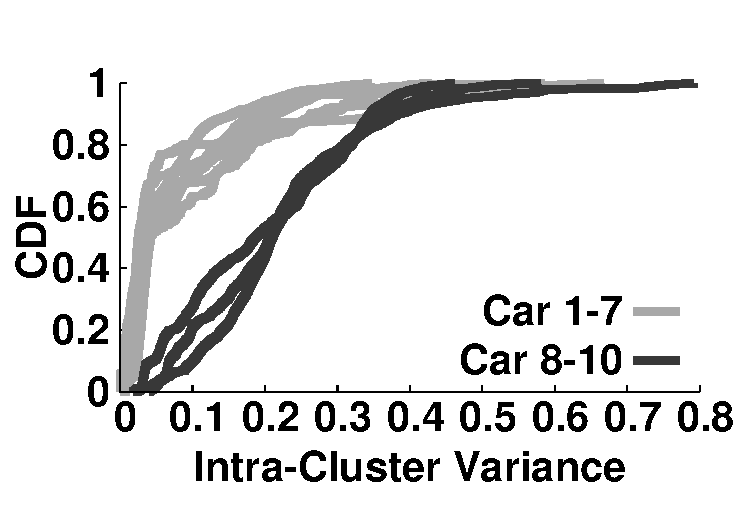
\includegraphics[width=1.7in,angle=0]{Figs/DriveSense/variance_cars.pdf}
\hspace{-0.5cm}
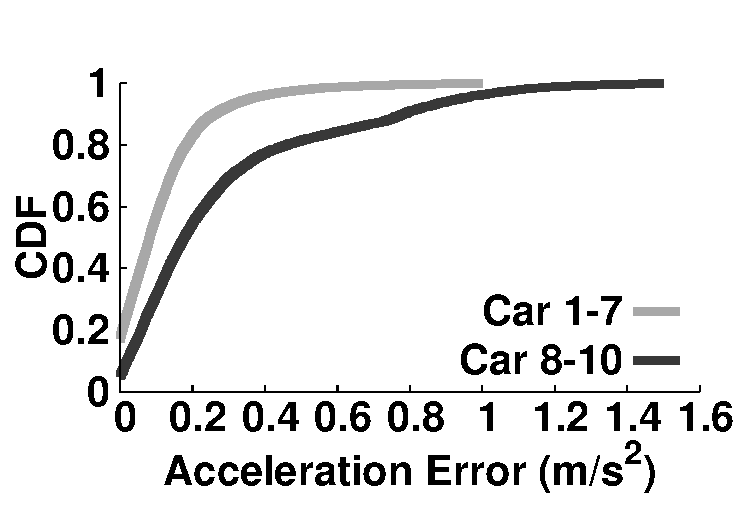
\includegraphics[width=1.7in,angle=0]{Figs/DriveSense/sensor_error_cars.pdf}
\vspace{-0.2cm}
\caption{The intra-cluster variance distribution of the tight group (car 1-7)
	and the loose group (car 8-10), and 
the estimated acceleration accuracy of the tight group is higher than those
	of the loose group.}
\vspace{-0.2cm}
\label{mounting}
\end{center}
\end{figure}


Another factor affects the accuracy of vehicle motion sensing
is the mounting stability of the smartphone. 
The stability of the smartphone depends on how the 
smartphone is fixed/placed/held in the car. 
A good case scenario is the user placing the smartphone
on a stable car mount holder. 
A bad case scenario is the user or passenger playing
motion games such as car racing which requires rotating
the smartphone. 
The derived sensor readings of the car are over noisy
due to shaking and/or rotating of the smartphone. 


We model one fixed relative orientation as a cluster of 
sensor readings. 
We use \emph{intra-cluster variance (ICV)} to estimate 
the stability of the smartphone.  
A stable mounting of the smartphone is expected to produce a smaller
variance than unstable holding by hands.  
Since ICV is correlated with the cluster
size, we use the ICV of the subclusters to represent
the ICV of the whole cluster. 
We define one subcluster is any continous $n$ 
points of the whole cluster.  
We use ICV to evaluate the mounting
stability of the tablets from dataset $\#1$. 
We firstly remove all the trips that there is orientation 
change detected. 
As shown in Fig. \ref{mounting}, 
all the data from the 10 cars are naturally divided into two groups, 
where the first group (car 1-7) has a median variance less than 0.05
and the second group (car 8-10) has a median variance around 0.2.
We name the first group as \emph{tight group} and 
the second one as \emph{loose group}. 
Since the tablets are not aligned with the cars, 
we conduct coordinate alignment and linear acceleration
estimation by using the methods in Section \ref{slopeaware}. 
We compare the acceleration estimated by aligned accelerometer
and the groundtruth acceleration calculated by OBD speed. 
As indicated in Fig. \ref{mounting}, 
the estimated accuracy of the tight group is generally higher
than the loose group. 


  





\section{The Promise of GPS in Driving Analytics}
\label{gps}


GPS is the most ubiquitous localization system and generally
provides absolute coordinates. 
The usability of GPS in driving analytics has not been 
well discussed by the communities due to its high energy cost 
and coarse-grained measurements. 
Our measurements indicate GPS is a good 
candidate especially when IMU sensor
is not available to use or less accurate. 
We find that GPS has high accuracy in 
estimating speed and accelerations, 
especially in high speed scenarios (e.g., >10m/s).  
Given the simplicity of acceleration estimation
and high accuracy of GPS, 
we believe inertial sensors can be 
augmented by GPS in vehicle speed and acceleration
estimation applications. 




\nop{
Recently, Google announced that the raw data (e.g., pseudoranges, Dopplers and carrier phase) 
of GPS receiver is accessible for Android 7.0 \cite{android_gnss, google_gnss_tools}. 
}

\subsection{How GPS Works}

GPS provides a simple way to track vehicle motions
due to its orientation independent nature.
However, it has been blamed for its low
accuracy \cite{hedgecock2013high, gowda2016tracking}.
A GPS receiver can compute the instant absolute location
by receiving ephemeris data transmitted from satellite systems. 
The GPS satellites transmit signal with the starting 
time of the transmission (obtained from the satellites' atomic clock). 
Meanwhile, the ground receiver records the time of reception with 
smartphone local clock. 
The flight-time is the gap between these timestamps. 
The major error is caused by the smartphone GPS receiver
clock biases \cite{hedgecock2013high, gowda2016tracking}. 
Considering we are interested in the relative position of 
two continuous measurements from the same GPS receiver, 
the clock biases of the measurements are neutralized. 
In this work, we use smartphone built-in GPS as 
an augmenting method for driving analytics. 
We leave the performance gain by utilizing GPS raw data for the future work.


\subsection{Speed Estimation}

\begin{figure}[!htbp]
\begin{center}
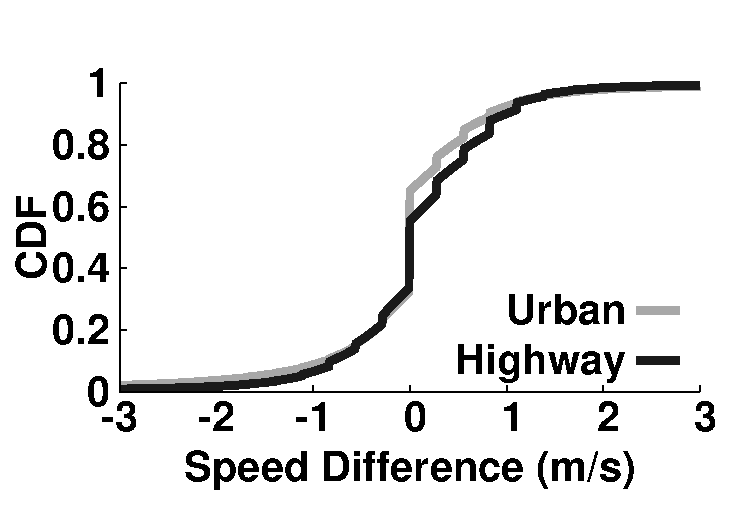
\includegraphics[width=2.6in,angle=0]{Figs/DriveSense/gpsobd_speed_diff.pdf}
\vspace{-0.2cm}
\caption{The speed estimation error of GPS.}
\vspace{-0.2cm}
\label{speeddiff}
\end{center}
\end{figure}

Speed calculation is very important for many vehicular applications \cite{hansenspeed, chandrasekaran2010vehicular}.  
GPS can provide speed information by simply calculating
the distance and time difference between two adjacent points. 
We use dataset $\#1$ (more details in section \ref{evaluation}) to evaluate the speed estimation of GPS. 
We tag the dataset with highway trips and urban trips,
based on speed distributions. 
Trips with a speed over $50mph$ in any segment is classified into highway trips. 
The CDF of speed estimation errors are plotted in Fig. \ref{speeddiff}. 
More than $90\%$ of the points are able to accurately calculate the speed 
with the error less than $1m/s$. 


\subsection{Acceleration Estimation}



\begin{figure}[!tb]
\begin{center}
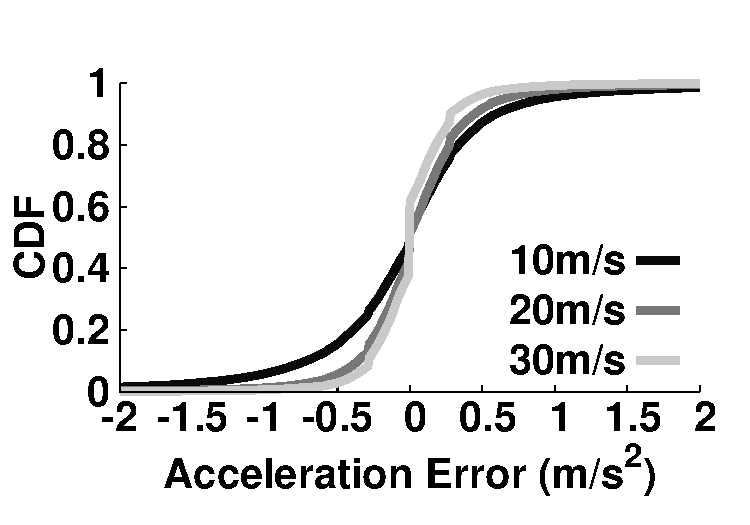
\includegraphics[width=3.0in,angle=0]{Figs/DriveSense/gpsobd_acce_speed.pdf}
\vspace{-0.2cm}
\caption{Acceleration estimation errors of GPS in urban and highway environments. 
	The estimation is more accurate in higher speed ($>10m/s$) than lower speed ($<10m/s$).}
\vspace{-0.2cm}
\label{accediff}
\end{center}
\end{figure}


The acceleration is comparatively evaluated by GPS points and OBD speed data.  
The CDF of estimation error is shown in Fig. \ref{accediff}. 
Each curve stands for the acceleration estimation error no more than that speed, i.e., 
$10m/s$ refers to any speeds not higher than $10m/s$ and $20m/s$ refers to any speeds between $10m/s$ and $20m/s$. 
The estimation errors of GPS in low speed are caused by GPS location estimation errors, which could be caused by either the weak GPS satellite signal or strong thermo-noise floor. 
Additionally, the errors could also be caused by the building and vehicle blockage.  
The acceleration estimation when the vehicular speed is higher than $20m/s$ 
is highly accurate. 
This result indicates that GPS is more accurate in high speed scenarios.




\subsection{GPS Availability}



\begin{figure}[!tb]
\begin{center}
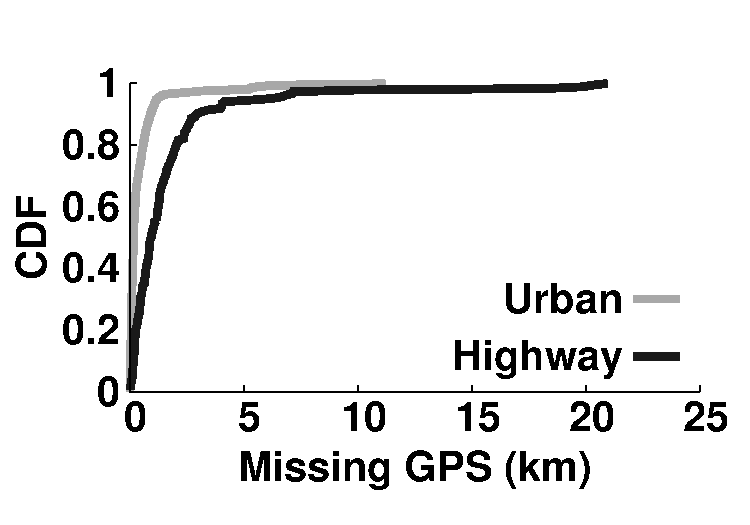
\includegraphics[width=1.7in,angle=0]{Figs/DriveSense/missing_gps.pdf}
\hspace{-0.5cm}
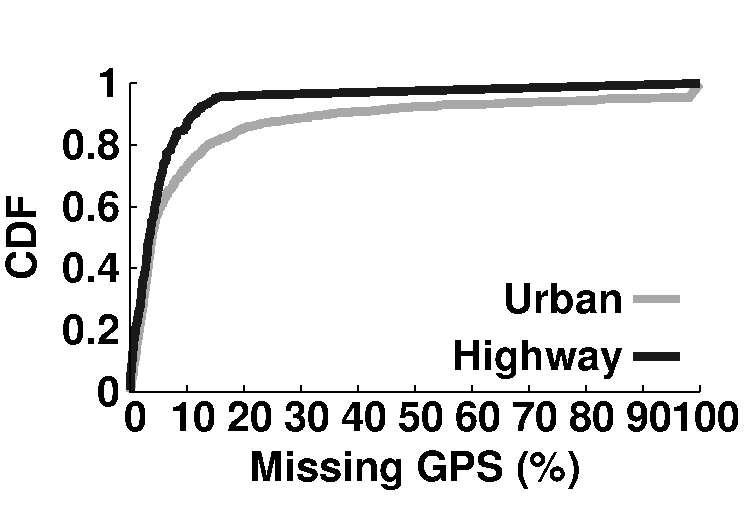
\includegraphics[width=1.7in,angle=0]{Figs/DriveSense/missing_percent.pdf}
\vspace{-0.2cm}
\caption{GPS availability in urban and highway environments. }
\vspace{-0.2cm}
\label{missinggps}
\end{center}
\end{figure}


GPS signal is not always available, especially in indoor
environments.
If the smartphone is inside the car, there are chances
that the smartphone GPS receiver is not able 
to detect satellite signals.  
Also, if the car is passing through underground tunnel or high buildings, 
GPS signal might be too weak to be received. 
We compare GPS and OBD data point by point, 
and record the accumulated distance of trip fragment without GPS points. 
The missing GPS of each trip is illustrated in Fig. \ref{missinggps}. 
There are a couple of trips that are entirely missing, 
while we are not sure if it is caused by software bugs or blocked signals. 
The GPS is available most of the time, while there are cases
that the GPS is missing at the start and/or end of the trip. 




 


%%%%%%%%%%%%%%%%%%%%%%%%%%%%%%%

\nop{
\subsection{Steering Angle Estimation}

\begin{figure}[!htbp]
\begin{center}
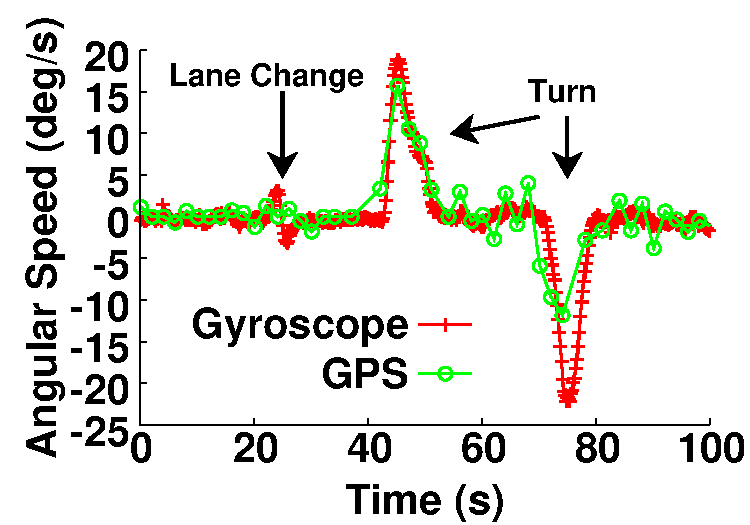
\includegraphics[width=2.6in,angle=0]{Figs/DriveSense/angular_illustration.pdf}
\vspace{-0.2cm}
\caption{An illustration of steering angular velocity estimation of GPS.}
\vspace{-0.2cm}
\label{steeringillustration}
\end{center}
\end{figure}

\begin{figure}[!htbp]
\begin{center}
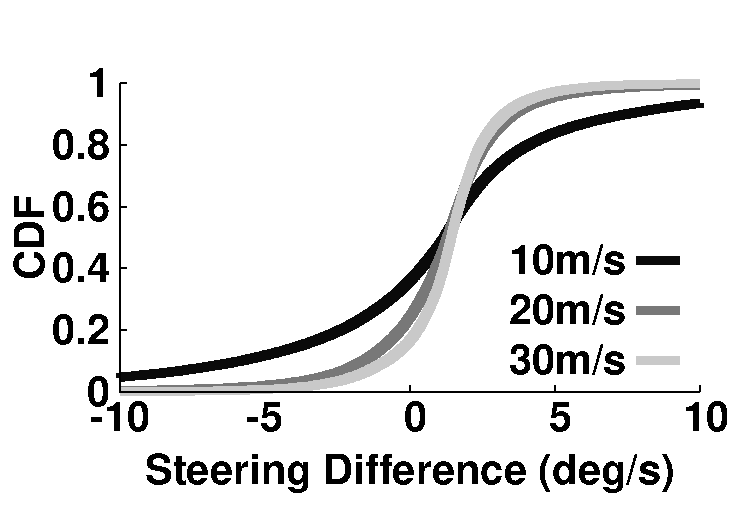
\includegraphics[width=2.6in,angle=0]{Figs/DriveSense/gps_steering.pdf}
\vspace{-0.2cm}
\caption{The GPS steering angular velocity estimation difference comparing with gyroscope.}
\vspace{-0.2cm}
\label{steeringdiff}
\end{center}
\end{figure}

Another important aspect of vehicle motion is steering motion. 
GPS can be used to estimate the changes of steering angle
by using a two pass processing. 
The first pass is used to calculate the moving direction
based on two GPS point. 
The second pass is used to calculate the angular attitude
rate based on direction differences. 
There are more noises on GPS readings
in low speed, i.e., the GPS indicates the vehicle is 
moving while the car is actually not, or the vehicle is stable but the GPS indicate the movement. 
Using adjacent points to calculate the direction introduces
lots of noises. 
We use the next GPS point at least $l-meter$ 
away as the next hop to calculate the direction. 
We compare the angular attitude rate estimated by GPS with
the ones estimated by 
gyroscope.
A trip fragment is illustrated in Fig.\ref{steeringillustration}
and the statistics are plotted in Fig. \ref{steeringdiff}.
Three observations can be concluded from this two Figs/DriveSense. 
First, the steering angular velocity estimated by GPS
is very coarse-grain, and cannot be used
for small direction movement such as lane changes. 
To detect the lane change, a precision of $0.5deg/s$ 
is required, while more than $80\%$ of the 
estimation error (by GPS) is higher than $1deg/s$.
Second, GPS can be used to identify large direction
changes such as turns, e.g., GPS can detect $83.54\%$
of the turns detected by gyroscope. 
GPS is very noisy when steering around parking lot
and cannot used for motion detection. 
Third, similar to acceleration estimation, 
the estimation accuracy of angular velocity is higher 
in high speed scenarios. 
}





\section{Design and Implementation}
\label{design_implement}




\subsection{Design of XSense}


\subsubsection{Workflow}

\begin{figure}[!htbp]
\begin{center}
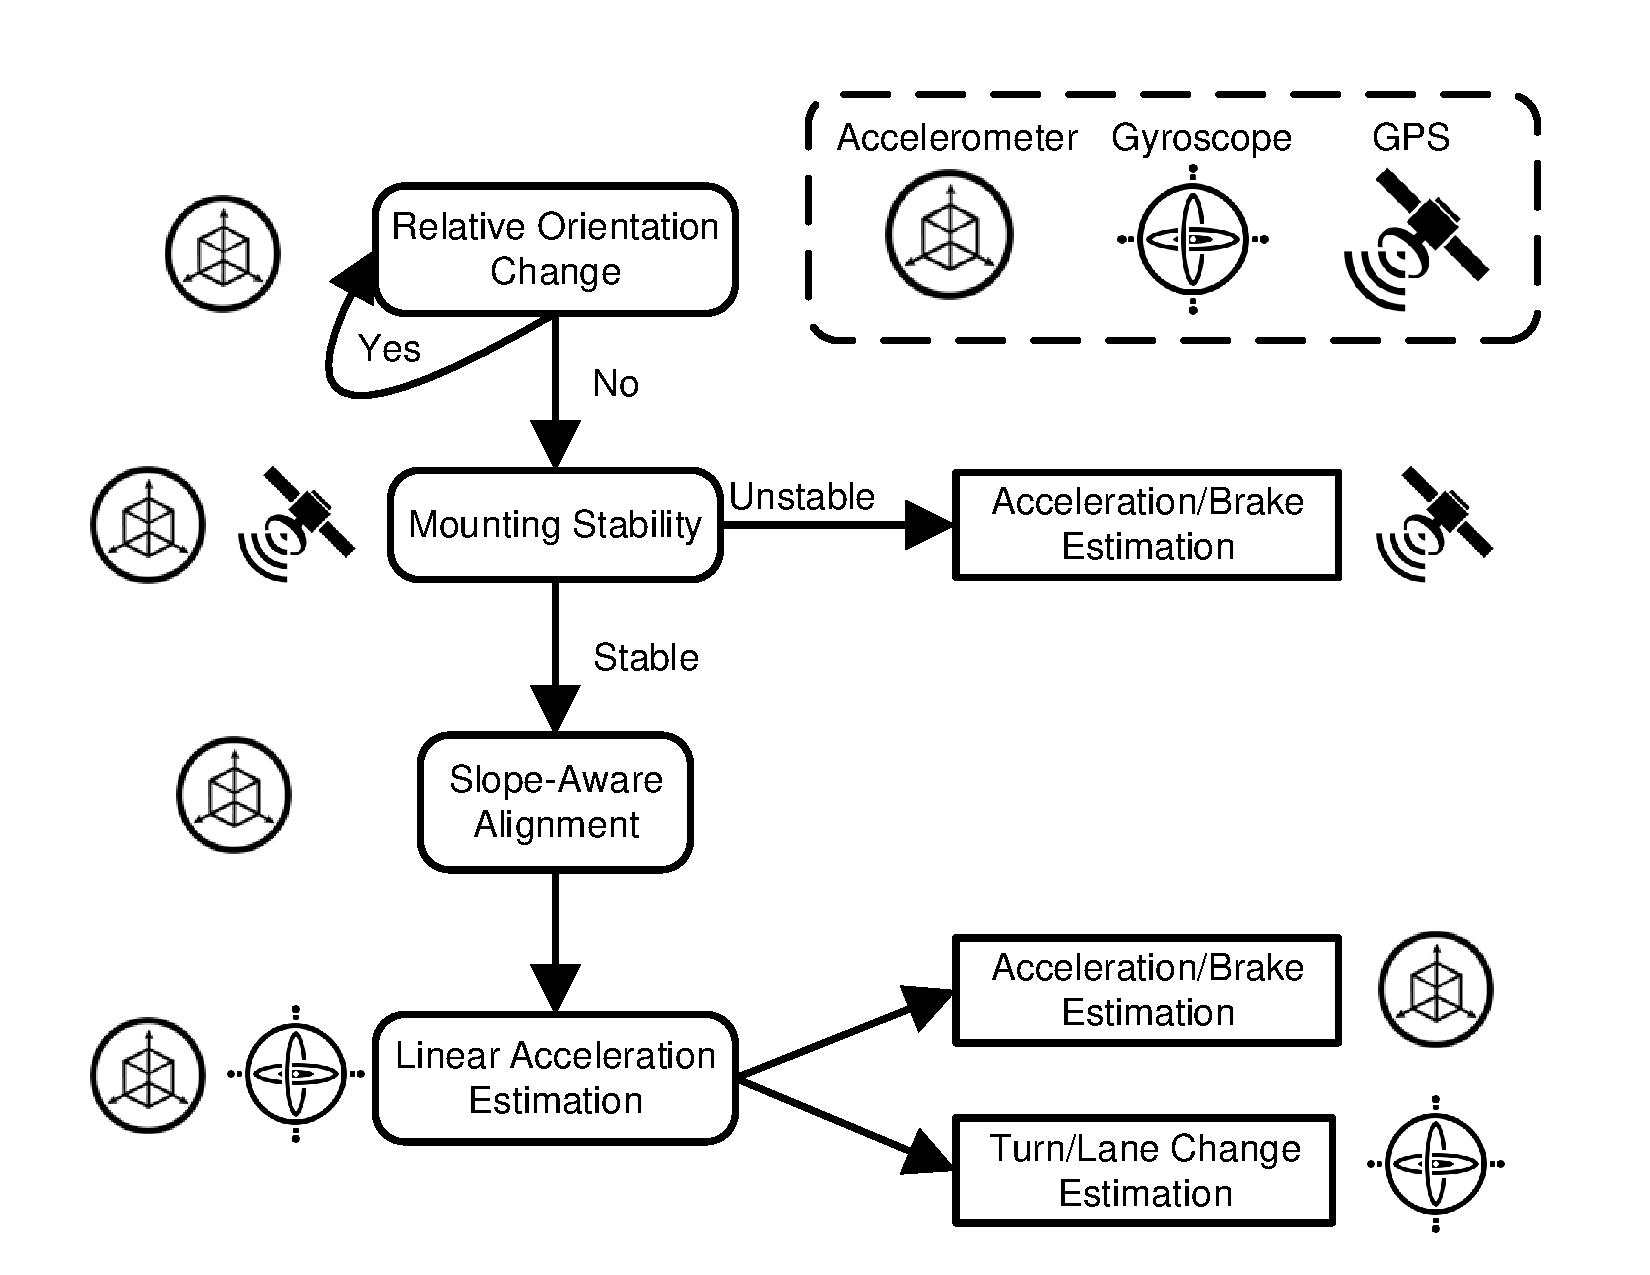
\includegraphics[width=3.6in, angle=0]{Figs/DriveSense/system_flowchart.pdf}
\vspace{-0.2cm}
\caption{Workflow of XSense.}
\vspace{-0.6cm}
\label{workflow}
\end{center}
\end{figure}


The workflow of XSense is illustrated in Fig. \ref{workflow}. 
XSense uses several modules to evaluate sensor
performance and estimate vehicle motion paramters. 
The inputs of XSense are accelerometer, gyroscope
and GPS.  
In each module, it uses different sensors as input.  
The corresponding sensor icon is placed along with the 
module if it requires that sensor as input.  
Our method uses the accelerometer extensively
as it provides a baseline by measuring the absolute acceleration while
the gyroscope measures only relative angular speed. 
The first module is to detect relative orientation changes.  
If an orientation change is detected, 
XSense will restart the rotation matrix
training process until the 
relative orientation of the phone is fixed.  
The second module is called stability monitoring
module, which is used to monitor the mounting
stability of the smartphone. 
The stability of the smartphone is quantified
by a threshold, which depends on the 
accuracy of GPS and that of the accelerometer. 
If the accuracy of the accelerometer is higher
than that of GPS, we think the smartphone
is mounted stably. 
In other case, we use GPS to estimate acceleration.
The third one is slope-aware coordinate
alignment module, 
which aligns the coordinates from the smartphone
to those of the car and estimates
the gradients of the training road segment. 
Both horizontal and vertical alignment are conducted
in this module. 
The last one is the linear acceleration estimation
module, which is used to estimate the slope 
gradients along the way.
XSense may selective use GPS or accelerometer
to estimate accelerations based on
the accuracy of each method. 
The accuracy comparison between GPS and accelerometer
is illustrated in section \ref{evaluation}. 



\subsubsection{Fusion with GPS}


GPS can be used to detect accelerations and brakes
when the IMU sensors are not available or not
ready to be used. 
IMU sensor is not available when the user 
frequently changes the relative orientation of the smartphone
or does not mount the smartphone stably. 
For example, if the user is holding the smartphone
to play game or send text message, 
the IMU sensor readings are too noisy 
to use. 
Even the user mounts the smartphone in a 
fixed place, it takes tens of seconds to minutes 
to collect enough data for training the rotation matrix. 
During the training process, the 
IMU sensors are not ready to be used.  
\footnote{The accelerometer takes much longer than gyroscope
as the gyroscope does not sense gravity.}


The GPS can also be used to eliminate the movement of the vehicle
when modeling mounting stability. 
We subtract the acceleration measured by the GPS from
the acceleration measured by the accelerometer. 
To do this, we project the 3D acceleration measured
by accelerometer into 2D space. 
Ideally, one dimension of senses gravity and the other
senses the horizontal movement of the car. 
For simplicity, we projects the 2D horizontal 
acceleration sensed by the accelerometer
into a single dimension and use it to subtract the acceleration
measured by GPS. 
We use this method only when the speed measured by GPS
is higher than a threshold. 


\subsection{Implementation}


We implement XSense as a software module in Java and 
import it to an Android application we wrote.
To make our test easier, we develop an offline 
trace replay engine.
The replay engine sorts the sensor data
based on timestamps, and feeds them into an event listener function in chronological order. 
We use an abstraction called \emph{Trace} to represent the sensor data, 
GPS data and OBD parameters.
It is similar to SensorEvent used by Android API \cite{sensor}
and provides additional flexibility to store OBD and GPS data. 
The event listener function process each \emph{Trace} 
according to corresponding sensor type.  
The trace replay engine makes it easier to import
XSense to the Android application. 
The Android application is aiming to monitor and record
daily driving trips. 
The app is implemented by less than 4,000 lines of Java code, 
but supports a variety of functionalities such as
trip recording, real time display, trip management,
trip display on Google map, user management and access control, 
online/offline uploading, data synchronization with remote server etc. 
XSense serves as a module that provide an more accurate
estimation on vehicle motions, e.g., hard brakes. 
For this submission, we highlight XSense module 
and remove some functionalities such as
trip upload, user management etc.
The QR code for a link to download the xsense.apk package is provided in Fig. \ref{xsense_app}. 

\begin{figure}[!tb]
\begin{center}
%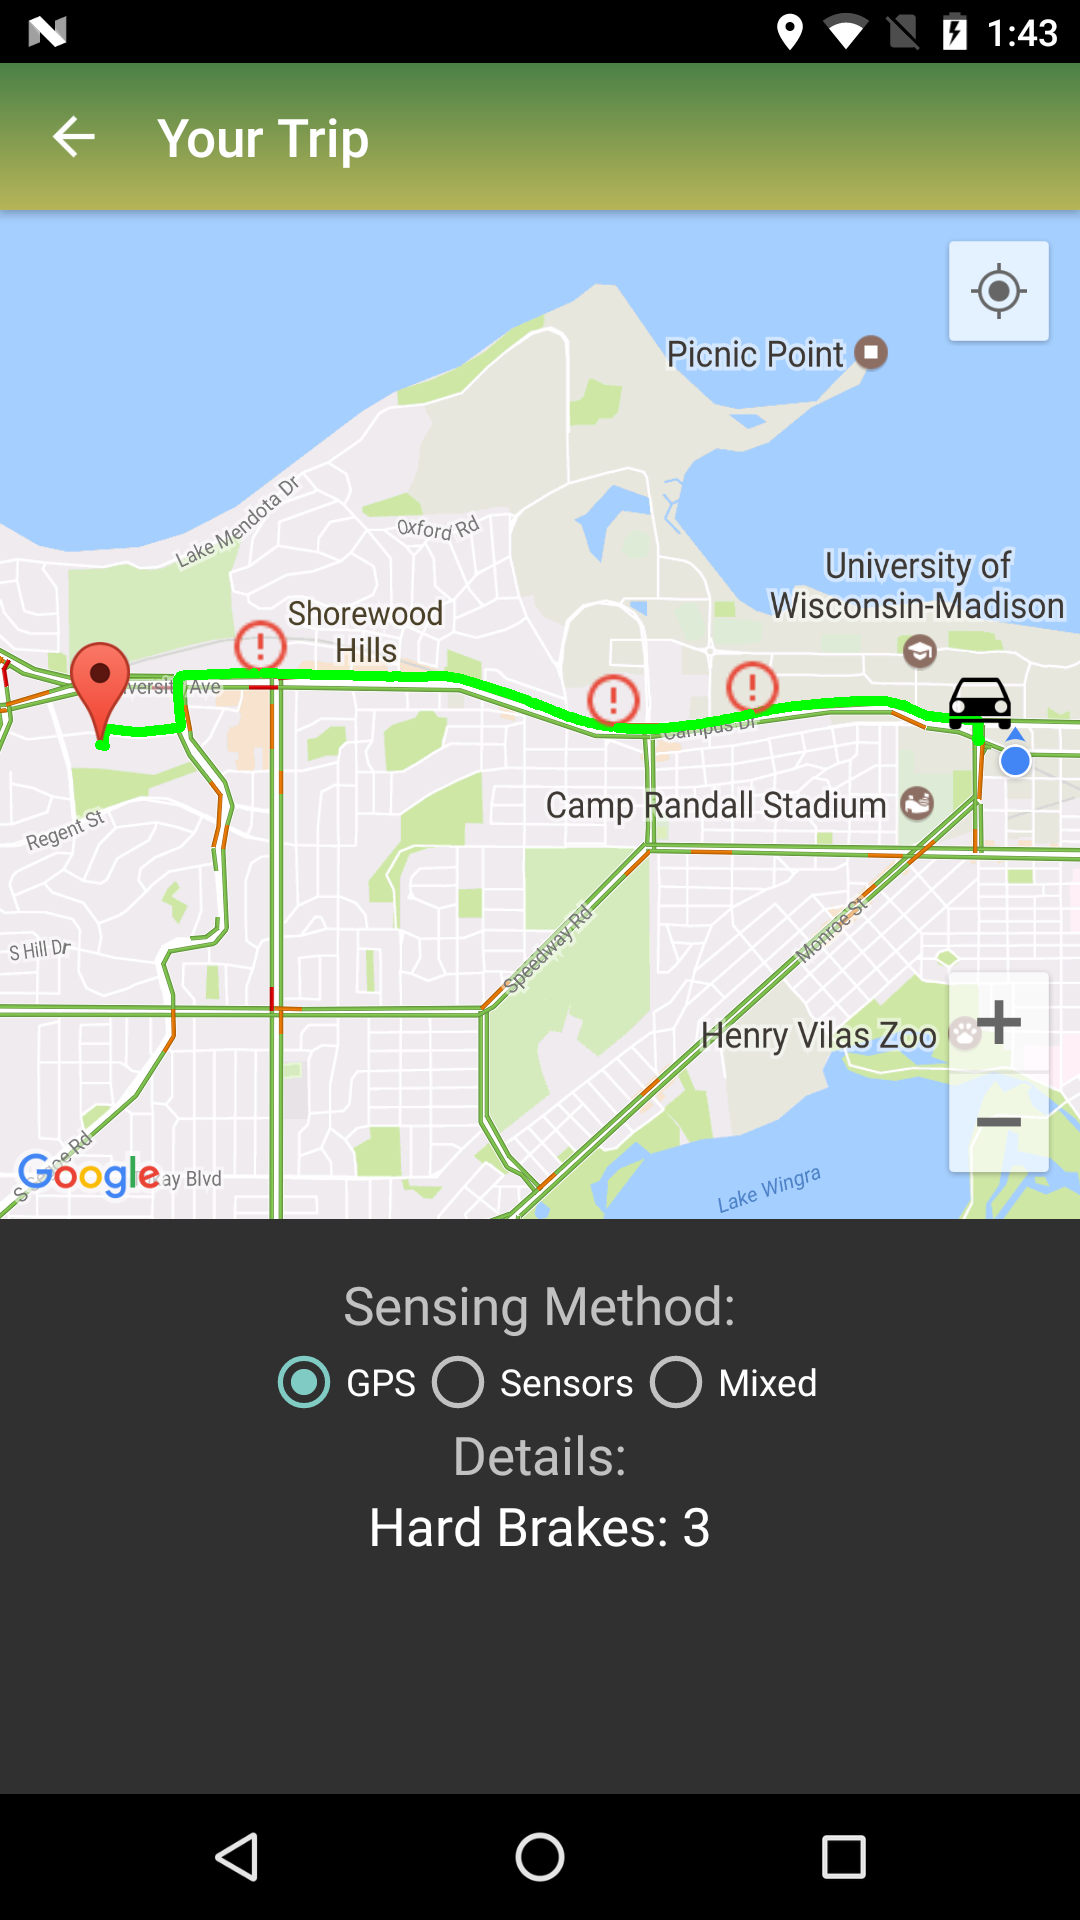
\includegraphics[width=1.7in,angle=0]{Figs/DriveSense/screenshot_gps.png}
%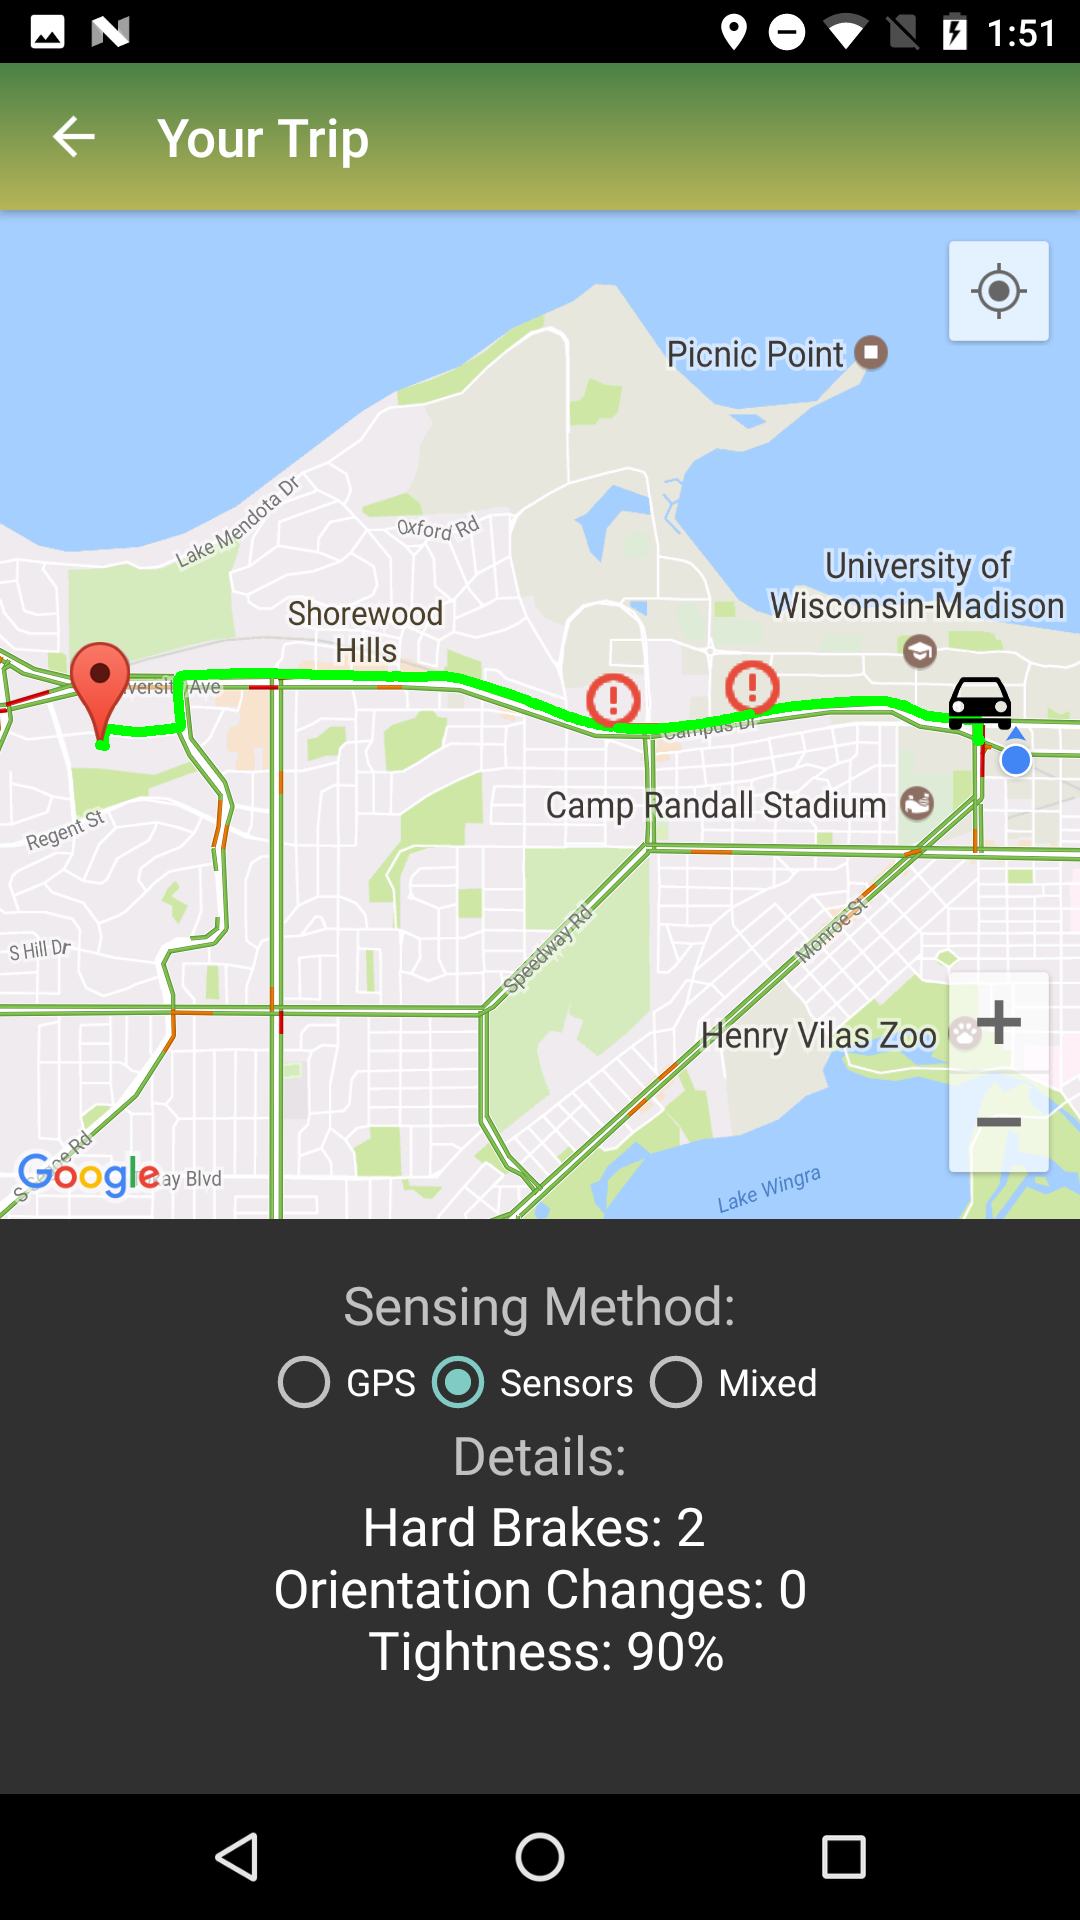
\includegraphics[width=1.7in,angle=0]{Figs/DriveSense/screenshot_sensors.png}
%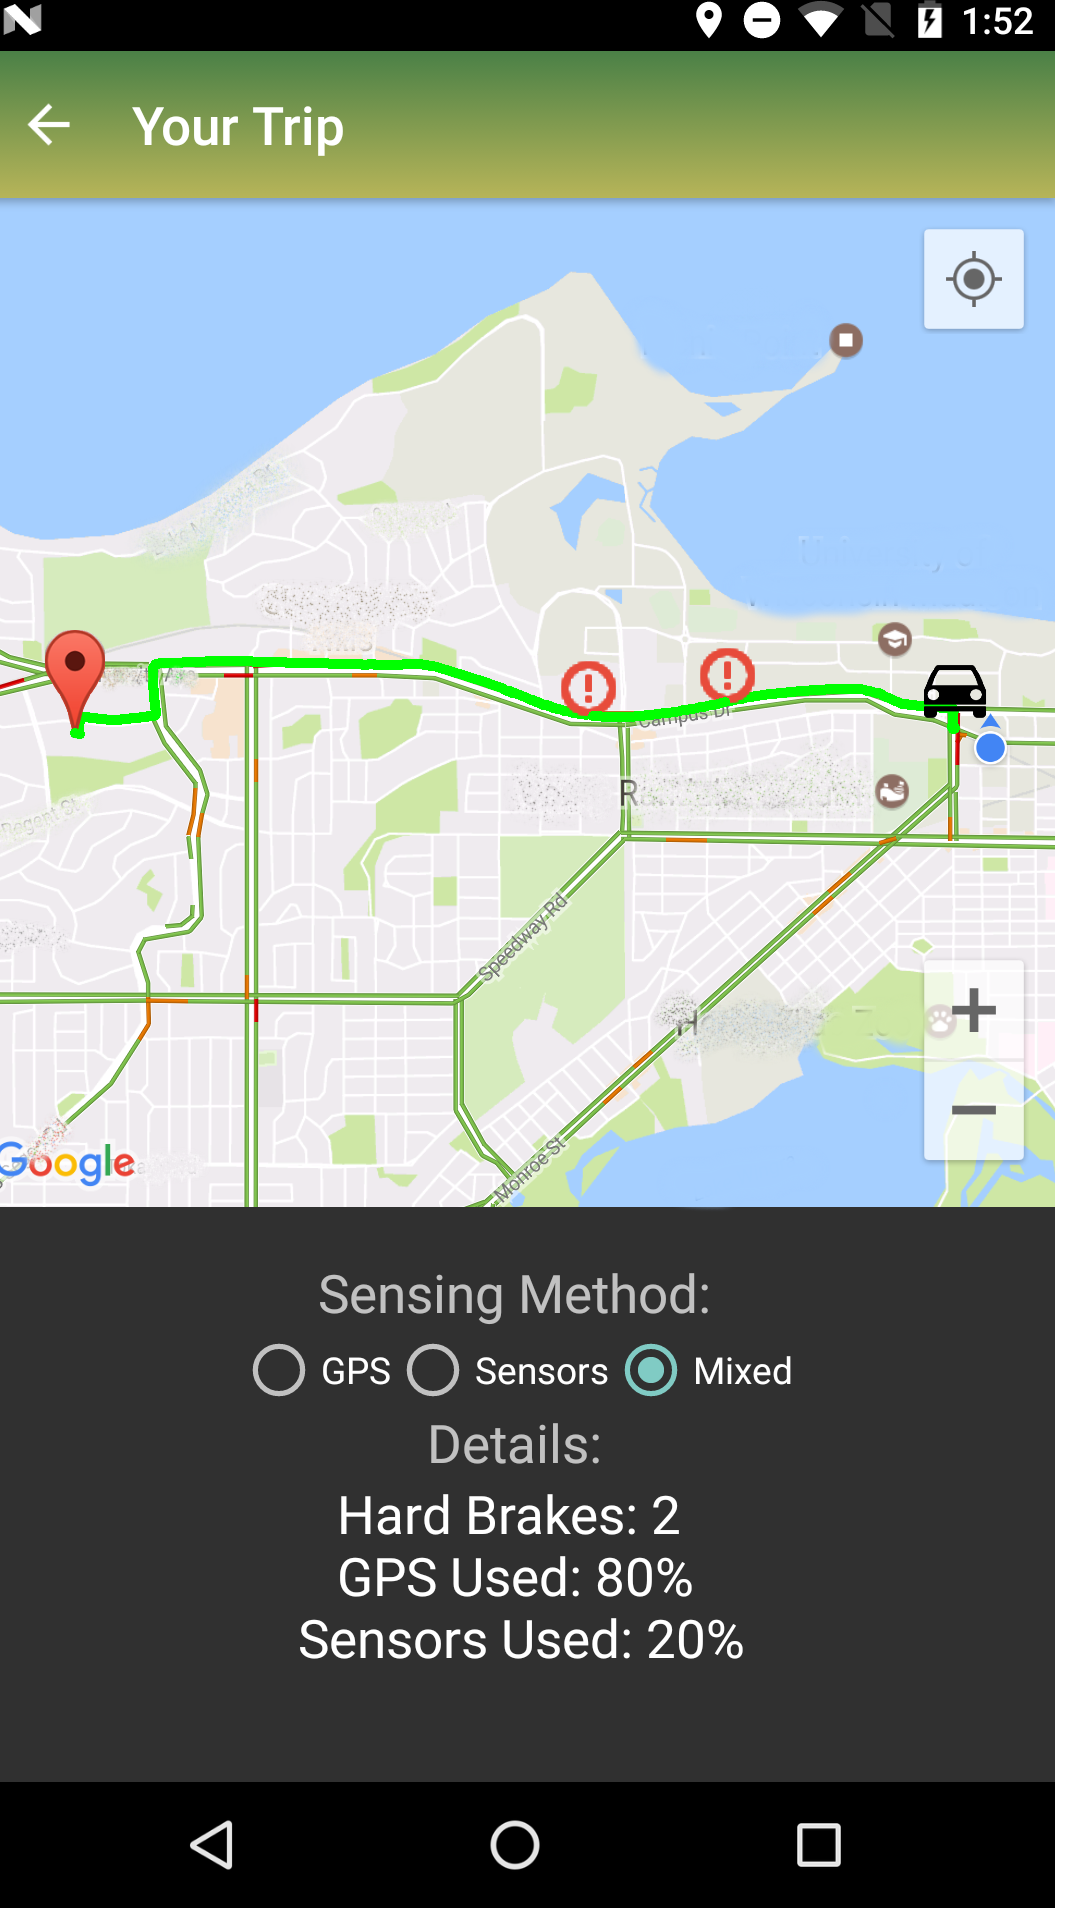
\includegraphics[width=1.8in, angle=0]{Figs/DriveSense/screenshot_mixed_hidden.png}
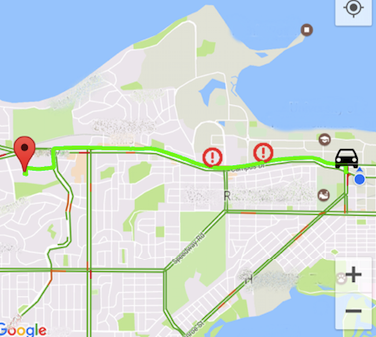
\includegraphics[width=1.8in, angle=0]{Figs/DriveSense/cut_app.png}

\includegraphics[width=1.4in, angle=0]{Figs/DriveSense/qrcode_xsense.png}
	\vspace{0.0cm}
\caption{The screenshot of XSense that user can view the hard brakes
	detected by GPS, sensors or mixed. The QR code can be scanned 
	to download the .apk Android installation file.}
\vspace{-0.2cm}
\label{xsense_app}
\end{center}
\end{figure}





\section{Experimental Results}
\label{evaluation}


\subsection{Dataset}

We use three datasets in our study. 
All of the datasets are collected by a gradually 
improved Android app.  
There are totally more than 13,000 miles of driving data 
collected in both controlled and uncontrolled environments
over the past three years.  
We will make our dateset available to public after 
this work has been published.  


\textbf{Dataset $\#1$}. 
We deploy Xoom tablets installed with our app on 10 different cars. 
The tablets collect the vehicular speed data from the On-board diagnostics (OBD)
port and various sensor data (including GPS and inertial sensors).  
Each tablet is placed in the back pocket of the passenger seat. 
The invovled cars are from different models and the stability
of the tablet placement is different, 
which provides the opportunity to study the effects of 
mounting stability on motion estimation accuracy.   


\textbf{Dataset $\#2$}.
We also collect some data in more controlled environments, 
where we know what is happening and the groundtruth data are recorded. 
First, we collect the data when the smartphone is placed in various scenarios, 
i.e., holding by hand, fixed by car mount holder, placed in cup holder etc. 
These data are used to understand various orientations and 
the relation between mounting stability and motion estimation accuracy.  
Second, we collect some data when randomly changing the 
orientation of the smartphone, i.e., 
move the smartphone from pocket and fix it on car mount holder. 
These data are used to evaluate the accuracy of 
our orientation change detection module. 
Third, we collect some data from two devices, where one device
is manually aligned with the car (as best as we can), 
and the other is fixed in car mount holder or held in passenger's hand. 
These data are used in two cases. 
One trip is used to understand acceleration
overestimation problem caused by gravitational force. 
Another 10 trips are used to estimate the
vehicle steering motions, where the gyroscope readings 
of manually aligned device is used as groundtruth data. 
 

\textbf{Dataset $\#3$}. 
We release the beta version of the Android app 
to 9 volunteers. 
The trip recording module is written as an Android Service,
so it is running in the background while the user may use 
the smartphone for navigation, game or any other activities. 
These data are used to understand how different users
are placing their smartphones while driving or 
sitting in the car. 



\subsubsection{Road Slope Statistics}

\begin{figure}[!htbp]
\begin{center}
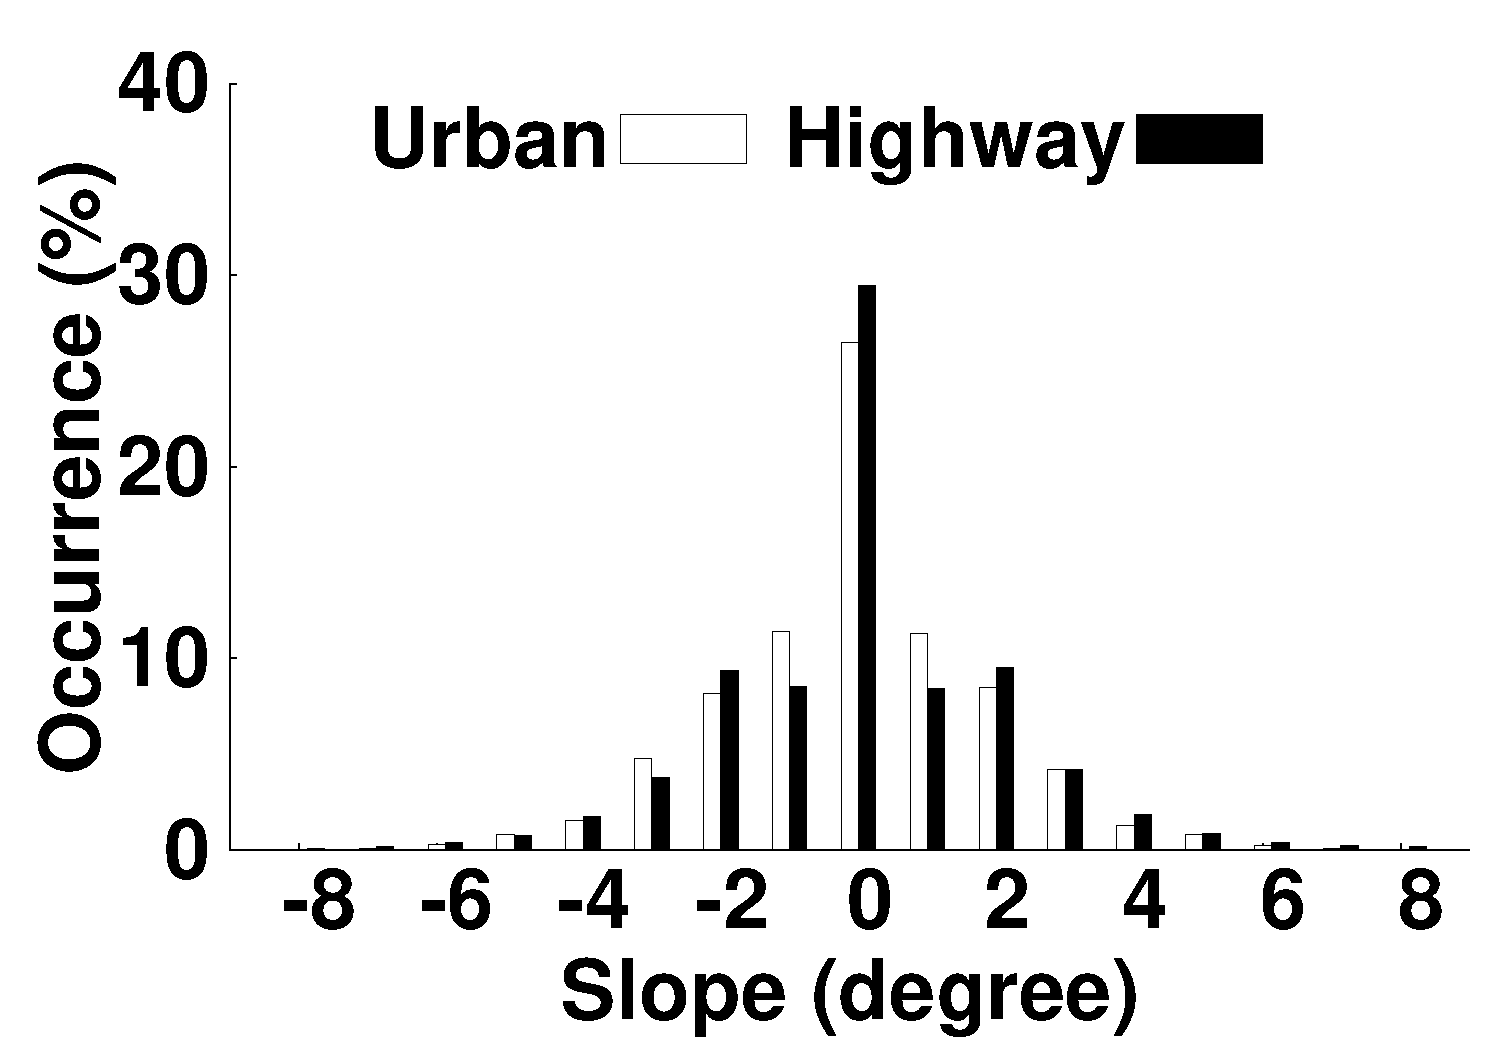
\includegraphics[width=2.5in, angle=0]{Figs/DriveSense/slopeaware/degrees.pdf}
%\hspace{-0.6cm}
%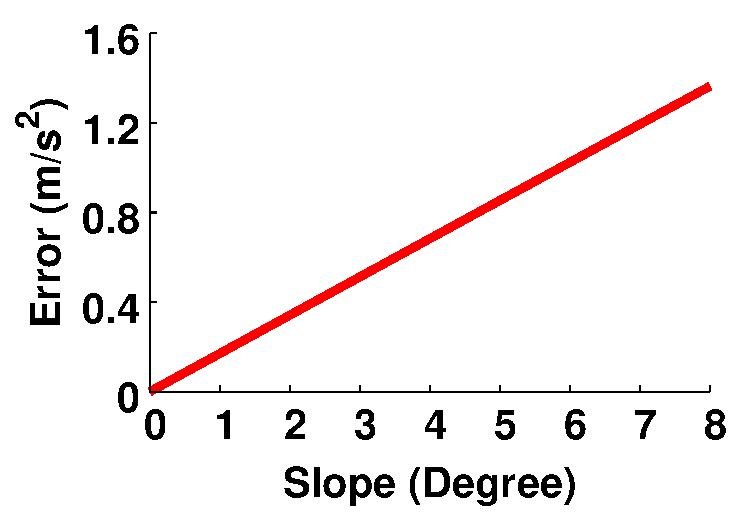
\includegraphics[width=2.5in, angle=0]{Figs/DriveSense/slopeaware/slope_error.pdf}
%\vspace{0.0cm}
%\caption{Histogram of slope gradients (left) and acceleration estimation errors 
%	under different slope gradients (right).}
\caption{Histogram of slope gradients. The acceleration estimation error is 
proportional to $gsin\theta$, where $\theta$ is the road slope angle.}
\label{slopegradients}
\vspace{-0.4cm}
\end{center}
\end{figure}


As we discussed above, the slopes introduce linear acceleration estimation errors.
An important question is how many road segments are sloping and
how many of them are actually level. 
Some cities, e.g., San Diego and Los Angeles, are full of hills, 
and most roads are sloping roads.
Surprisingly, in a plain area in US where we collect data, 
there are also full of slopes. 
To obtain the road gradient, we use the Google elevation dataset \cite{googleelevation}. 
For each GPS data point, we queried the elevation from the dataset. 
and calculated the gradient by the elevation difference
and distance.
We eliminated the close consecutive GPS data points that less than 5 meters in distance and removed the data points where the speed is less than $10mph$.
As we can see from the histogram in Fig. \ref{slopegradients}, 
more than half of the roads are not flat.
Those sloping roads, even as small as two degrees, may introduce accumulated
errors on coordinate alignment and further slope estimation, i.e., $0.34m/s^2$.
The aggregated error may cause significant linear acceleration estimation error
and introduce false positives/negatives on brake/acceleration monitoring. 




\subsection{Improved Overall Accuracy}

\subsubsection{Acceleration Estimation}


We use dataset $\#1$ to evaluate the accuracy of DriveSense and
other methods. 
The other three methods are using Accelerometer with Traditional Coordinate
Alignment (TCA)  \cite{hansenspeed, wang2013sensing, chen2015invisible}, 
Slope-Aware coordinate alignment with linear 
acceleration estimation, 
and GPS.
In this evaluation, we only use the tight group data where the 
tablet is stably fixed in the car.  
Therefore, the results generated by sensors are 
the best cases can be achieved for sensor-based motion estimations. 
We compare the acceleration difference between
each method and the groudtruth (calculated by OBD speed). 
The results are shown in Fig. \ref{xsense_accuracy}. 
The estimation made by well-tuned sensor coordinate alignment and 
linear acceleration estimation (Slope-Aware curve)
shows similar $80\%$ accuracy with GPS. 
The gap between Slope-Aware and Accelerometer are caused
by road slopes, 
where slope-unaware solution will over/under-estimate 
acceleration due to gravitational force. 
The accuracy gain of DriveSense is from the 
acceleration estimation compensation by sensors
when the GPS speed is low. 

 

\begin{figure}[t]
\begin{center}
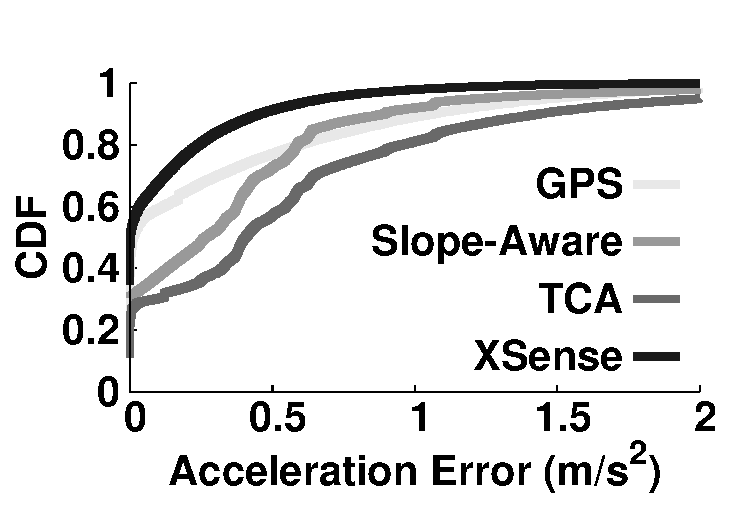
\includegraphics[width=3.0in,angle=0]{Figs/DriveSense/evaluation/xsense_accuracy.pdf}
\vspace{-0.2cm}
\caption{Comparing acceleration estimation accuracy among various methods.}
\vspace{-0.3cm}
\label{xsense_accuracy}
\end{center}
\end{figure}





\subsubsection{Steering Angular Velocity Estimation}


\begin{figure}[!htbp]
\begin{center}
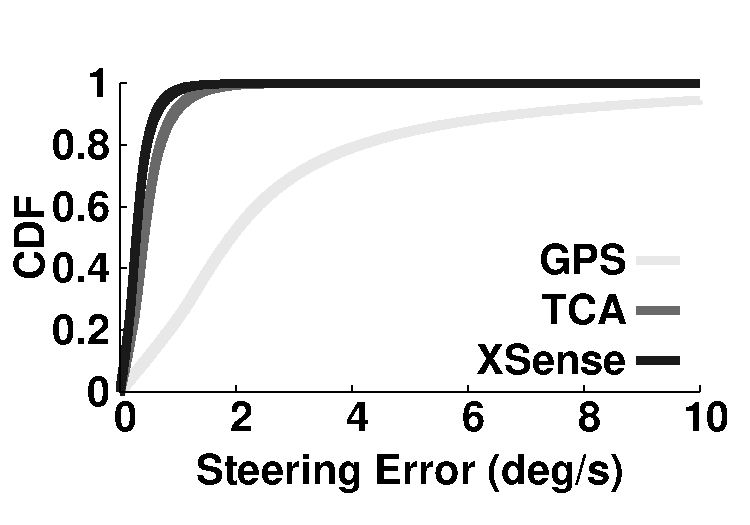
\includegraphics[width=3.0in,angle=0]{Figs/DriveSense/evaluation/evaluation_steering.pdf}
\vspace{-0.2cm}
\caption{Comparing steering angular velocity estimation accuracy among various methods. }
\vspace{-0.3cm}
\label{xsense_steering}
\end{center}
\end{figure}

We use dataset $\#2$ to evaluate steering angular velocity 
estimations. 
In this setting, one device is manually aligned with
the car and the gyroscope reading of which is used
as the groundtruth. 
Another device is fixed in car mount holder.    
As expected and can be seen in Fig. \ref{xsense_steering}, 
GPS can not estimate angular velocity accurate enough
for small horizontal movement such as lane change due to
its large estimation errors. 
DriveSense performs slightly better than gyroscope with 
Traditional Coordinate Alignment (TCA) due to 
the slope-aware solution presented in this work. 
The gain is obtained in the cases where the coordinate
alignment is conducted on slope, and there is vertical
misalignment caused by slope-unaware coordinate alignment. 




\subsection{Orientation Change Detection}

We evaluate the orientation change module
by using dataset $\#2$ in this section. 


\textbf{Detection Rate}.
The performance of inertial sensors in vehicle
motion sensing applications highly depends
on the fixed relative orientation between
the smartphone and the car. 
Therefore, detecting orientation change is 
very important in such applications. 
We evaluate the orientation change detection methods 
in two settings, tight setting and loose setting. 
In tight setting, the smartphone is mounted in 
various orientations on the car mount holder, 
or mounted by car cup holder. 
In loose setting, the smartphone is put in 
pocket, placed in passenger seat, or holding by 
passenger's hand. 
For each orientation, we record 
the groundtruth by a customized app. 
We use more than 10 trips and record
98 orientation changes in tight setting 
and 82 orientation changes in loose setting. 
The detection rate is presented in Table \ref{evaluate_change}. 
The Moving Variance method can detect most
of the orientation changes expect when 
there is small horizontal orientation change. 
But such orientation change will increase the 
Intra-Cluster Variance so that the stability 
detection module can identify
the polluted sensor output. 


\begin{table}[!htbp]
        \vspace{0.5cm}
        \centering
        \caption[evaluate_change]{Orientation Change Detection Accuracy}
         \vspace{0.0cm}
        \label{evaluate_change}
                \begin{tabular}{|l|c|c|}
                \hline
Method & Tight & Loose
\\  \hline      \hline
MV & $96.9\%$  &  $87.8\%$ 
\\  \hline
MV + ICV & $100\%$ & $96.3\%$   
\\  \hline
     \end{tabular}
\end{table}


%98 orientation changes
%95 detected with both
 
%82 loose orientaiton changes
%72 detected



\begin{figure}[!htbp]
\begin{center}
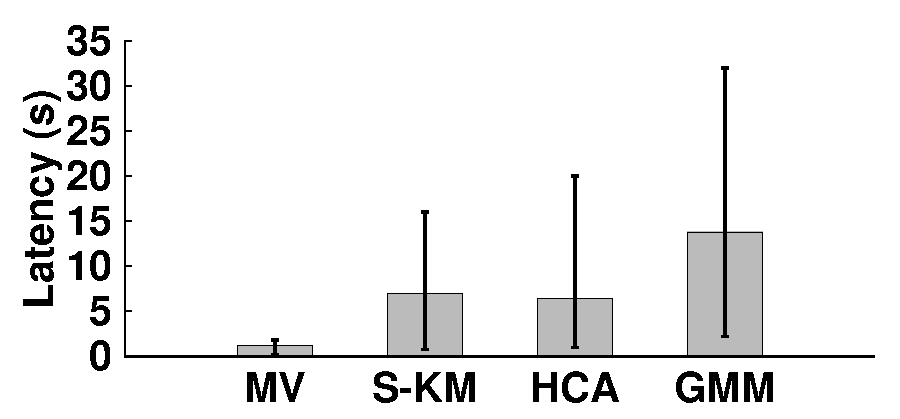
\includegraphics[width=3.0in,angle=0]{Figs/DriveSense/clustering_methods.pdf}
\vspace{0.0cm}
\caption{The time used to detect there is an orientation change.}
\vspace{-0.2cm}
\label{evaluate_latency}
\end{center}
\end{figure}


\textbf{Detection Latency}. 
Detecting orientation change timely can reduce possible inaccurate 
estimations. 
We compare the moving variance (MV) method with other common
data stream clustering method such as 
sequential K-means (SK), hierarchical clustering (HCA) 
and Gaussian Mixture Models (GMM). 
We run the four methods in 10 different orientation changes, 
and the results are shown in Fig. \ref{evaluate_latency}. 
MV can detect orientation change in 10-20 data samples (1-2s). 
The common incremental clustering techniques require more
time as it needs more data to form/detect another cluster. 



\subsection{Comparison Between GPS and IMU Sensors}

\begin{figure}[!htbp]
\begin{center}
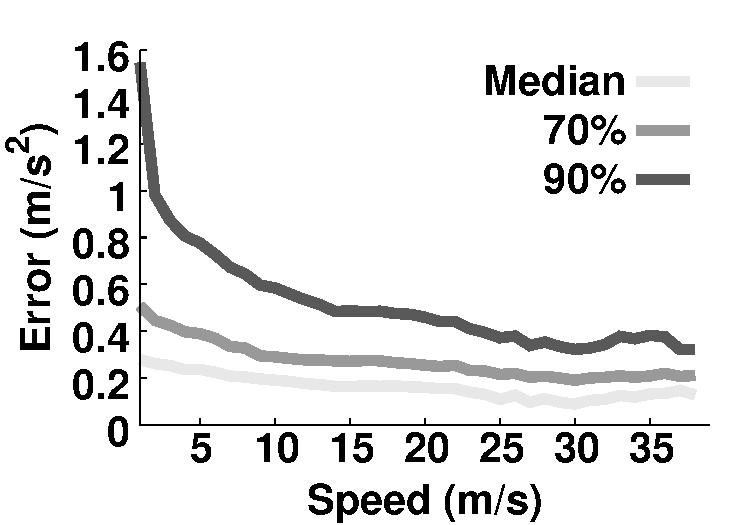
\includegraphics[width=3.0in, angle=0]{Figs/DriveSense/speed_acce_error.pdf}
\vspace{-0.2cm}
\caption{GPS acceleration estimation errors under various speeds.}
\vspace{-0.4cm}
\label{speed_acce_error}
\end{center}
\end{figure}




\begin{table}[!htbp]
        \centering
        \vspace{0.5cm}
        \caption[icv_accuracy]{Median ICV and Acceleration Estimation Accuracy}
         \vspace{0.0cm}
        \label{icv_accuracy}
                \begin{tabular}{|l|c|c|c|}
                \hline
ICV Median & Median Error & $70th-\%$ & $90th-\%$ 
\\  \hline      \hline
0.05 & $0.15m/s^2$  & $0.18m/s^2$ & $0.31m/s^2$ 
\\  \hline
0.21 & $0.21m/s^2$  &  $0.38m/s^2$ & $0.95m/s^2$   
\\  \hline
0.87 & $0.45m/s^2$ & $0.78m/s^2$ & $1.56m/s^2$   
\\  \hline
\end{tabular}
\end{table}


To select between IMU sensor and GPS as input
for acceleration estimation, 
we compare the accuracy based on current speed and 
mounting stability. 
To estimate the accuracy of GPS, 
we use one pipeline to process GPS stream data 
and track the speeds. 
Each GPS point is associated with a confidence value. 
The confidence value is the $\beta$$th$ percentile
estimation accuracy under given speed.
The percentile accuracy under various speeds
is illustrated in Fig. \ref{speed_acce_error}.
To estimate the accuracy of IMU sensors, 
we use ICV to track the mounting stability of the smartphone. 
We use the median ICV as an indicator of
the mounting stability. 
The corresponding percentile errors of different
ICV are illustrated in Table \ref{icv_accuracy}.



\subsection{Training Time}

\begin{figure}[!htbp]
\begin{center}
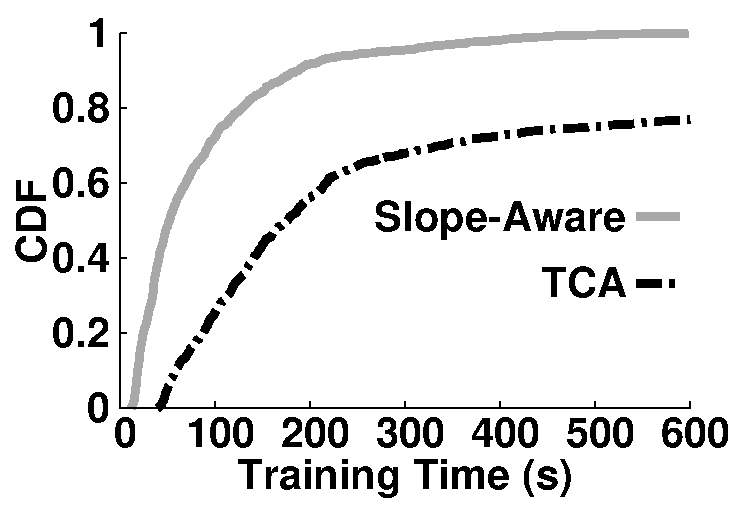
\includegraphics[width=2.8in,angle=0]{Figs/DriveSense/slopeaware/alignment.pdf}
\vspace{-0.2cm}
\caption{The training time used for coordinate alignment.}
\label{alignmenttime}
\vspace{-0.3cm}
\end{center}
\end{figure}

The training time of a coordinate alignment algorithm is critical
for real-time applications such as hard brake warning \cite{snapshot}. 
To evaluate the training time, we extract the straight road driving segments and fed them into the replay engine.
The engine stops when the accuracy of coordinate alignment is within
a predefined percentage of the accuracy when we use the segments of the entire trip to train.
As shown in Fig. \ref{alignmenttime}, 
there is a substantial improvement on the training speed.
Slope-aware alignment matrix can be trained in less than $2min$ in more than
$80\%$ of the cases, 
while it takes much longer time to train the rotation matrix if
the algorithm does not consider slope caused deviations.
The training time heavily depends on road conditions. 
For the trips with level roads and fewer bumps, it generally
takes less time to train.
On the other hand, for the trips with lots of slopes and bumps on the road, 
it takes much longer time to train due to less training opportunities.


\subsection{In the Wild}


%\subsubsection{Statistics}

\begin{figure}[!htbp]
\begin{center}
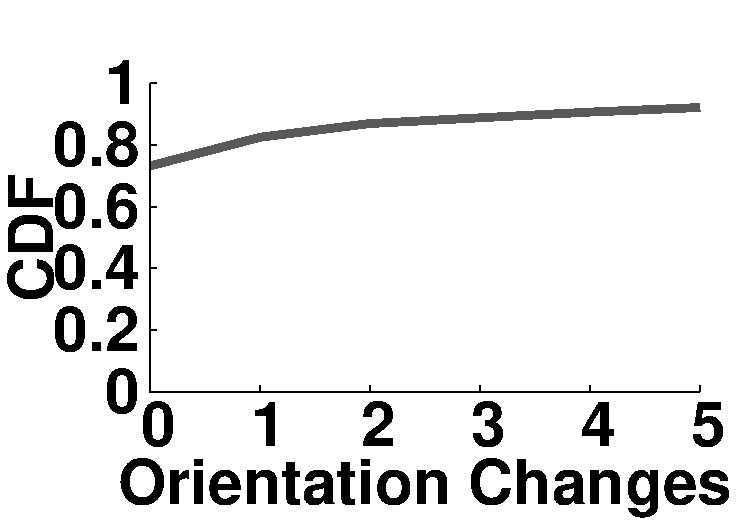
\includegraphics[width=1.7in,angle=0]{Figs/DriveSense/evaluation/wild_changes.pdf}
\hspace{-0.5cm}
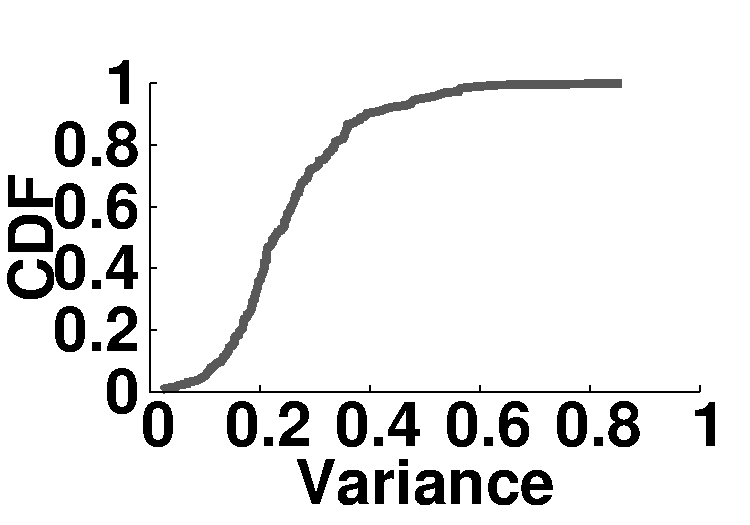
\includegraphics[width=1.7in,angle=0]{Figs/DriveSense/evaluation/wild_variances.pdf}
\vspace{0.0cm}
\caption{The orientation change and stability measurement statistics.}
\vspace{-0.2cm}
\label{wild_evaluation}
\end{center}
\end{figure}


The beta version of our Android application (the full version with 
trip upload, user management and back-end server etc.) is released to
9 volunteers for the past half year. 
There are totally 269 trips collected. 
The trip recording functionality of the app is designed as an Android 
Service, so it is able to run in the background. 
We observe some users forget to stop the app, 
so we add another functionality to stop recording if there
is no high speed movement in 10 minutes. 
The volunteers are asked to place the Android phone
at anywhere they prefer. 
Among the 269 trips we collected, 
orientation change occurs in 74 trips. 
The CDF of the orientation change statistics are 
illustrated in Fig. \ref{wild_evaluation}.
Normally it takes about several minutes to find a fragment
to train the rotation matrix, frequent changing 
the orientation may reduce the opportunities using
inertial sensors. 
We also evaluate the stability or the variance of the trips 
without orientation changes. 
The results, as shown in Fig. \ref{wild_evaluation}, 
indicate that the smartphones are mounted tightly
in most of cases. 
There are about $25\%$ trips where the smartphone is not 
tight enough (high variances) and GPS should be used instead. 


\nop{
\subsubsection{Parameter Selection}

\begin{figure}[!htbp]
\begin{center}
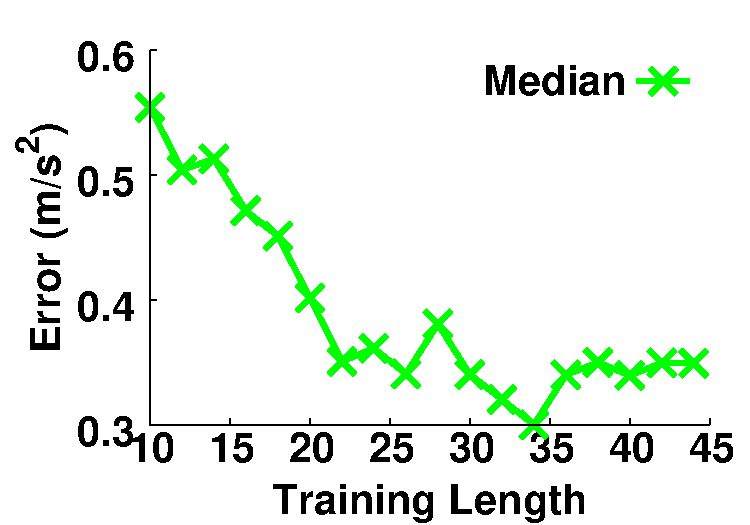
\includegraphics[width=1.7in,angle=0]{Figs/DriveSense/trainlengthanderror.pdf}
\vspace{0.0cm}
	\caption{The training length is related to horizontal alignment median error.}
\label{training}
\vspace{-0.2cm}
\end{center}
\end{figure}
}







\section{Limitation and Discussion}


\textbf{Extra Power Consumption of GPS}. 
The use of GPS will accelerate the power consumption of the smartphone. 
We believe user experience is more important
than power consumption within vehicle, 
where the user is able to charge the smartphone. 
We find that some vehicle travel recording applications, like DriveWell \cite{cmt} , monitoring GPS information
in the background. 
We believe the users are willing to enjoy some 
vehicle service such as navigation and travel recording
in exchange for some extra power.  



\textbf{Better or Worse GPS accuracy}. 
Our GPS evaluation is limited to existing techniques as well as the
geographic scope where we collected the data. 
The GPS has a chance to perform better with more advanced algorithms
or worse with signals blocked by high buildings. 
Google has implemented the API which allow the application layer to use raw GNSS data as input
since Android 7.0 system \cite{android_gnss, google_gnss_tools}.
With extra input, we believe the accuracy of GPS in commodity 
smartphone could be improved. 
The accuracy of GPS in metropolitan cities could be decreased when vehicles are passing through high buildings blocking the GPS signal.
DriveSense is a system framework that can alternatively use the best estimation
Method.
With the training and modeling techniques presented in this paper, 
we believe DriveSense is able to accommodate new techniques.  

\textbf{High-end Vehicles}. 
There are emerging selfdriving techniques that ultilize 
expensive hardwares to scan the road, 
which may provide better accuracy on road condition
monitoring. 
Also they could be equipped with built-in sensors
and alignment is not a problem anymore. 
But our techniques about linear acceleration
estimation and fusion with GPS still work
in such cases. 
We argue that the majority of existing
vehicles are still low-end vehicles 
and we expect they will still dominate 
the road in the next decade. 
Our techniques can be used in either high-end 
or low-end vehicles by using only
a single smartphone. 


\textbf{Device and Orientation Diversity}. 
We are not able to try all the devices and 
every possible orientation. 
The devices we used include Motorola Xoom,
HTC Hero, LG Nexus 5, LG Nexus 5x and Motorola Nexus 6. 
The devices are placed in the back pocket of passenger
seat, vertically /horizontally in car mount holder, 
car cup holder, passenger seat, pants pocket, 
and passenger hand.  
We believe the diversity of devices and orientations in our study are representative enough. 
We have not observed neither particular device nor 
the orientation influence on vehicle motion sensing
with inertial sensors. 






\section{Summary of DriveSense}




Smartphones are commonly used for driving analytics applications. 
Traditional approaches assume experimental
cases where the smartphone is stably mounted with fixed relative orientation
and the vehicle is travelling on flat roads. 
By using an example experiment, we show that 
even perfectly aligned accelerometer suffers acceleration overestimation or underestimation, 
which is caused by gravitational force, misalignment and slope estimation error.  
Moreover, the accuracy of IMU sensors are sensitive to human interactions
as well. 
For example, frequent relative orientation change and less stable mounting
may cause significant estimation errors. 
In this work, the defects are remedied
with following innovative techniques. 
First, a slope-aware alignment algorithms to reduce the slope influence, 
meanwhile, to improve alignment accuracy. Also, we track the linear 
acceleration of the vehicle to address acceleration over/under estimation problems. 
Second, in order to timely update 
vehicular motion parameters, the relative orientation changes of 
smartphone are detected using machine learning algorithms. 
Third, we model mounting stability of the smartphone and 
evaluate the sensing accuracy under different stability estimations.  
Fourth, we present the tradeoffs between inertial sensors, the primary sensors, 
and GPS, which is used when inertial sensors lose accuracy or disable. 
To evaluate our solutions, we compare the estimated 
accelerations with those calculated from OBD speed readings.  
The accuracy of our methods are evaluated with highway and urban traces
covered by 13,000 miles in the northwestern US.
We show through our experiments and analysis that
compared to current state of the art techniques, 
our method improves the $75$-percentile accuracy 
by $5\times$ comparing with well-tuned inertial sensors in traditional approach. 






\begin{algorithm}
\caption{Angle Search Algorithm}
\label{search}
\begin{algorithmic}[1]
\Input{$D_a$: The 2D accelerometer data after horizontal alignment}
\Output{$\theta_{o}$: The best fit angle}
\Procedure{AngleSearch}{}
\State $dev_{min} \gets MAX$;
\State $D_{t} \gets []$;
\For{$\theta$ \texttt{in} (-$\alpha$, $\alpha$)}
\For{$[y_i, z_i]$ \texttt{in} $D_a$}
\State $M_\nu$ $\gets$ $\begin{bmatrix}\cos\theta & -\sin\theta\ \\ \sin\theta & \cos\theta \end{bmatrix}$;
\State $[y'_i,z'_i]$ $\gets$ $[y_i,z_i]* M_\nu$;
\State $D_t.push(z'_i)$;
\EndFor
\State $dev_x \gets deviation(D_t)$;
\If {$dev_x < dev_{min}$}
\State {$dev_{min}$ $\gets$ $dev_x$};
\State {$\theta_{o}$ $\gets$ $\theta$};
\EndIf
\EndFor
\Return $\theta_{o}$;
\EndProcedure
\end{algorithmic}
\end{algorithm}
\vspace{-0.6cm}




